\documentclass[11pt]{article}
\usepackage{fullpage,enumitem,amsmath,amssymb,graphicx,amsthm}
\usepackage{subcaption}
\usepackage{caption}
\usepackage{braket}
\usepackage{authblk}
\usepackage{tikz} 
\usetikzlibrary{arrows.meta, calc}
\usepackage{quantikz}
\usepackage{multicol}
\usepackage{float}

% --- 하이퍼링크 설정 ---
\usepackage{hyperref} 
\hypersetup{
    colorlinks=true,
    linkcolor=blue,
    filecolor=magenta,      
    urlcolor=cyan,
    citecolor=blue,
}

\usepackage{geometry}
\geometry{margin=1in}

\usepackage{style}

% --- 수학 환경(Theorem Environments) 설정 ---
\theoremstyle{definition}
\newtheorem{definition}{Definition}[section]
\newtheorem{example}{Example}[section]

\theoremstyle{plain}
\newtheorem{theorem}{Theorem}[section]
\newtheorem{corollary}{Corollary}[theorem] 
\newtheorem{proposition}{Proposition}[theorem]
\newtheorem{lemma}{Lemma}[theorem]

\theoremstyle{remark}
\newtheorem*{remark}{Remark}

\title{Abstract Algebra : A Brief Review}
\author{Jeongbin Jo}
\affil{Department of Physics, Yonsei University, \texttt{jeongbin033@yonsei.ac.kr}}

\begin{document}

\maketitle

\begin{abstract}
This document provides a comprehensive review of the fundamental concepts in abstract algebra, with a specific focus on group theory. It outlines the axiomatic definition of groups and distinguishes between abelian and non-abelian structures based on the law of composition. A variety of concrete examples, including the group of integers, all six rigid symmetries of an equilateral triangle ($D_3$), general linear groups with matrix operations, integers modulo $n$, and the quaternion group, are systematically explored to bridge abstract definitions with concrete mathematical objects. Finally, basic properties such as the order of a finite group and the formal proof regarding the uniqueness of the identity element are discussed.
\end{abstract}

\tableofcontents
\vspace{0.3cm}
\hrule
\vspace{0.5cm}

\section{Groups}

\subsection{Definition of a Group}

The concept of a group is central to abstract algebra, providing a unified framework for studying symmetries and generalized arithmetic operations.

\begin{definition}[Group]
A group $(G, f)$ is a set $G$ equipped with a map $f: G \times G \to G$, called a binary operation or law of composition, satisfying the following three axioms \cite{dummit, fraleigh}:
\begin{enumerate}
    \item \emph{Associativity:} For all $a, b, c \in G$, $f(f(a,b),c) = f(a,f(b,c))$ \cite{dummit}.
    \item \emph{Identity Element:} There exists an element $e \in G$ such that for all $a \in G$, $f(e,a) = a$ and $f(a,e) = a$ \cite{fraleigh}.
    \item \emph{Inverse Element:} For each $a \in G$, there exists an element $b \in G$ such that $f(a, b) = e$ and $f(b, a) = e$ \cite{dummit}.
\end{enumerate}
\end{definition}

\begin{remark}
It is a common and convenient convention to denote the binary operation $f(a,b)$ simply as $a \cdot b$ or $ab$ \cite{dummit}. Furthermore, a group $(G, f)$ is said to be \emph{abelian} (or commutative) if $f(a,b) = f(b,a)$ for all $a, b \in G$ \cite{gallian}.
\end{remark}

\subsection{Examples of Groups} 

The following examples illustrate various abstract group structures, expanding deeply into matrix groups and geometric symmetries.

\begin{example}[The Integers]
The set of integers $\mathbb{Z}$ together with standard addition forms a group denoted by $(\mathbb{Z}, +)$ \cite{fraleigh}. The identity element is $0$, since $a+0 = 0+a = a$ \cite{dummit}. The inverse of any integer $a$ is $-a$, yielding $a + (-a) = 0$ \cite{dummit}. This group is abelian \cite{gallian}.
\end{example}

\begin{example}[Symmetries of an Equilateral Triangle]
Symmetries are rigid transformations mapping the shapes back to itself, preserving both angle and distance. The set of all such symmetries for an equilateral triangle forms a group under the binary operation of composition \cite{gallian}. 

Let the initial vertices of the triangle be $A$ (bottom-left), $C$ (bottom-right), and $B$ (top). The group $G = \{id, \mu_1, \mu_2, \mu_3, \rho_1, \rho_2\}$ consists of exactly 6 elements \cite{dummit}:
\begin{itemize}
    \item \textbf{Reflections ($\mu$):} $\mu_2$ fixes $B$ and swaps $A, C$. $\mu_1$ fixes $A$ and swaps $B, C$. $\mu_3$ fixes $C$ and swaps $A, B$.
    \item \textbf{Rotations ($\rho$):} $\rho_1$ is a clockwise rotation by $120^\circ$. $\rho_2$ is a counter-clockwise rotation by $120^\circ$.
    \item \textbf{Identity ($id$):} Leaves the triangle completely unchanged.
\end{itemize}

\begin{figure}[h]
    \centering
    
    % ==========================================
    % 첫 번째 줄: mu_1 (A 고정 반사) | rho_1 (우측 120도 회전)
    % ==========================================
    \begin{minipage}{0.48\textwidth}
        \centering
        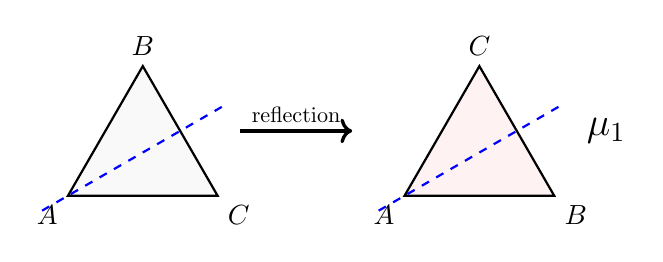
\begin{tikzpicture}[scale=0.95, thick]
            \coordinate (A1) at (-1, 0);
            \coordinate (C1) at (1, 0);
            \coordinate (B1) at (0, 1.732);

            \draw[fill=gray!5] (A1) -- (C1) -- (B1) -- cycle;
            \node[below left] at (A1) {$A$};
            \node[below right] at (C1) {$C$};
            \node[above] at (B1) {$B$};
            
            \draw[dashed, blue] (-1, 0) ++(210:0.4) -- ++(30:2.8);
            \draw[->, very thick] (1.3, 0.866) -- (2.8, 0.866) node[midway, above, scale=0.8] {reflection};
            
            \coordinate (A2) at (3.5, 0); 
            \coordinate (B2) at (5.5, 0); 
            \coordinate (C2) at (4.5, 1.732); 
            
            \draw[fill=red!5] (A2) -- (B2) -- (C2) -- cycle;
            \node[below left] at (A2) {$A$};
            \node[below right] at (B2) {$B$};
            \node[above] at (C2) {$C$};
            
            \draw[dashed, blue] (3.5, 0) ++(210:0.4) -- ++(30:2.8);
            \node[right, font=\Large] at (5.8, 0.866) {$\mu_1$};
        \end{tikzpicture}
    \end{minipage}\hfill
    \begin{minipage}{0.48\textwidth}
        \centering
        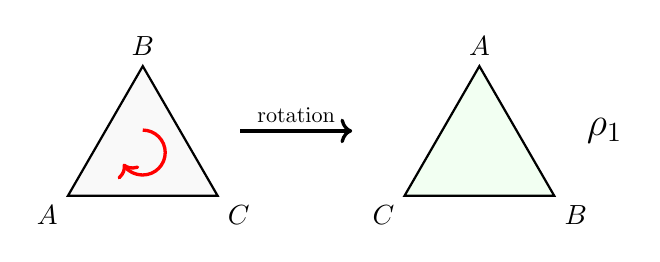
\begin{tikzpicture}[scale=0.95, thick]
            \coordinate (A1) at (-1, 0);
            \coordinate (C1) at (1, 0);
            \coordinate (B1) at (0, 1.732);

            \draw[fill=gray!5] (A1) -- (C1) -- (B1) -- cycle;
            \node[below left] at (A1) {$A$};
            \node[below right] at (C1) {$C$};
            \node[above] at (B1) {$B$};
            
            \draw[->, red, very thick] (0, 0.577) ++(90:0.3) arc (90:-150:0.3);
            \draw[->, very thick] (1.3, 0.866) -- (2.8, 0.866) node[midway, above, scale=0.8] {rotation};
            
            \coordinate (C2) at (3.5, 0); 
            \coordinate (B2) at (5.5, 0); 
            \coordinate (A2) at (4.5, 1.732); 
            
            \draw[fill=green!5] (C2) -- (B2) -- (A2) -- cycle;
            \node[below left] at (C2) {$C$};
            \node[below right] at (B2) {$B$};
            \node[above] at (A2) {$A$};
            
            \node[right, font=\Large] at (5.8, 0.866) {$\rho_1$};
        \end{tikzpicture}
    \end{minipage}

    \vspace{1cm} % 줄 사이 간격

    % ==========================================
    % 두 번째 줄: mu_2 (B 고정 반사) | rho_2 (좌측 120도 회전)
    % ==========================================
    \begin{minipage}{0.48\textwidth}
        \centering
        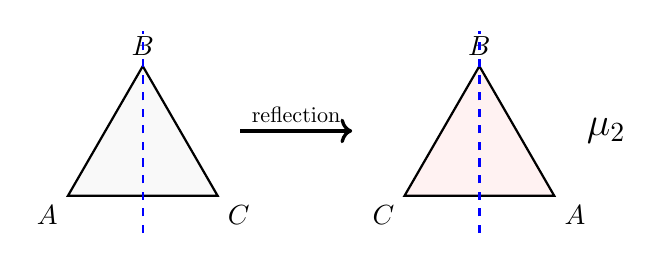
\begin{tikzpicture}[scale=0.95, thick]
            \coordinate (A1) at (-1, 0);
            \coordinate (C1) at (1, 0);
            \coordinate (B1) at (0, 1.732);

            \draw[fill=gray!5] (A1) -- (C1) -- (B1) -- cycle;
            \node[below left] at (A1) {$A$};
            \node[below right] at (C1) {$C$};
            \node[above] at (B1) {$B$};
            
            \draw[dashed, blue] (0, -0.5) -- (0, 2.2);
            \draw[->, very thick] (1.3, 0.866) -- (2.8, 0.866) node[midway, above, scale=0.8] {reflection};
            
            \coordinate (C2) at (3.5, 0); 
            \coordinate (A2) at (5.5, 0); 
            \coordinate (B2) at (4.5, 1.732); 
            
            \draw[fill=red!5] (C2) -- (A2) -- (B2) -- cycle;
            \node[below left] at (C2) {$C$};
            \node[below right] at (A2) {$A$};
            \node[above] at (B2) {$B$};
            
            \draw[dashed, blue] (4.5, -0.5) -- (4.5, 2.2);
            \node[right, font=\Large] at (5.8, 0.866) {$\mu_2$};
        \end{tikzpicture}
    \end{minipage}\hfill
    \begin{minipage}{0.48\textwidth}
        \centering
        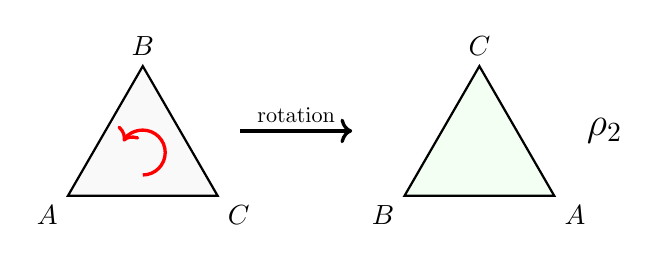
\begin{tikzpicture}[scale=0.95, thick]
            \coordinate (A1) at (-1, 0);
            \coordinate (C1) at (1, 0);
            \coordinate (B1) at (0, 1.732);

            \draw[fill=gray!5] (A1) -- (C1) -- (B1) -- cycle;
            \node[below left] at (A1) {$A$};
            \node[below right] at (C1) {$C$};
            \node[above] at (B1) {$B$};
            
            \draw[->, red, very thick] (0, 0.577) ++(-90:0.3) arc (-90:150:0.3);
            \draw[->, very thick] (1.3, 0.866) -- (2.8, 0.866) node[midway, above, scale=0.8] {rotation};
            
            \coordinate (B2) at (3.5, 0); 
            \coordinate (A2) at (5.5, 0); 
            \coordinate (C2) at (4.5, 1.732); 
            
            \draw[fill=green!5] (B2) -- (A2) -- (C2) -- cycle;
            \node[below left] at (B2) {$B$};
            \node[below right] at (A2) {$A$};
            \node[above] at (C2) {$C$};
            
            \node[right, font=\Large] at (5.8, 0.866) {$\rho_2$};
        \end{tikzpicture}
    \end{minipage}

    \vspace{1cm} % 줄 사이 간격

    % ==========================================
    % 세 번째 줄: mu_3 (C 고정 반사) | rho_3 (항등원)
    % ==========================================
    \begin{minipage}{0.48\textwidth}
        \centering
        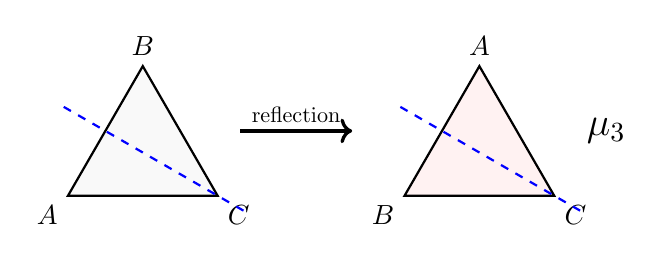
\begin{tikzpicture}[scale=0.95, thick]
            \coordinate (A1) at (-1, 0);
            \coordinate (C1) at (1, 0);
            \coordinate (B1) at (0, 1.732);

            \draw[fill=gray!5] (A1) -- (C1) -- (B1) -- cycle;
            \node[below left] at (A1) {$A$};
            \node[below right] at (C1) {$C$};
            \node[above] at (B1) {$B$};
            
            \draw[dashed, blue] (1, 0) ++(-30:0.4) -- ++(150:2.8);
            \draw[->, very thick] (1.3, 0.866) -- (2.8, 0.866) node[midway, above, scale=0.8] {reflection};
            
            \coordinate (B2) at (3.5, 0); 
            \coordinate (C2) at (5.5, 0); 
            \coordinate (A2) at (4.5, 1.732); 
            
            \draw[fill=red!5] (B2) -- (C2) -- (A2) -- cycle;
            \node[below left] at (B2) {$B$};
            \node[below right] at (C2) {$C$};
            \node[above] at (A2) {$A$};
            
            \draw[dashed, blue] (5.5, 0) ++(-30:0.4) -- ++(150:2.8);
            \node[right, font=\Large] at (5.8, 0.866) {$\mu_3$};
        \end{tikzpicture}
    \end{minipage}\hfill
    \begin{minipage}{0.48\textwidth}
        \centering
        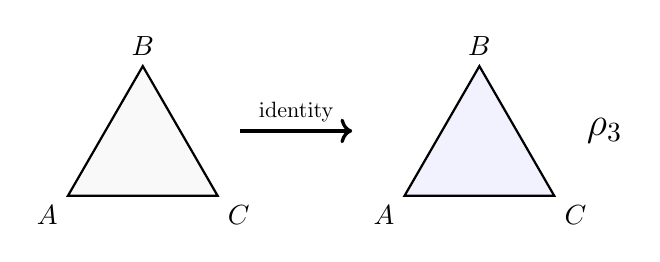
\begin{tikzpicture}[scale=0.95, thick]
            \coordinate (A1) at (-1, 0);
            \coordinate (C1) at (1, 0);
            \coordinate (B1) at (0, 1.732);

            \draw[fill=gray!5] (A1) -- (C1) -- (B1) -- cycle;
            \node[below left] at (A1) {$A$};
            \node[below right] at (C1) {$C$};
            \node[above] at (B1) {$B$};
            
            \draw[->, very thick] (1.3, 0.866) -- (2.8, 0.866) node[midway, above, scale=0.8] {identity};
            
            \coordinate (A2) at (3.5, 0); 
            \coordinate (C2) at (5.5, 0); 
            \coordinate (B2) at (4.5, 1.732); 
            
            \draw[fill=blue!5] (A2) -- (C2) -- (B2) -- cycle;
            \node[below left] at (A2) {$A$};
            \node[below right] at (C2) {$C$};
            \node[above] at (B2) {$B$};
            
            \node[right, font=\Large] at (5.8, 0.866) {$\rho_3$};
        \end{tikzpicture}
    \end{minipage}

    \caption{The six symmetry operations of an equilateral triangle, composing the Dihedral group $D_3$. Reflections ($\mu$) are arranged on the left, and rotations ($\rho$) are on the right.}
    \label{fig:all_symmetries_modified}
\end{figure}

The composition of these operations is non-abelian. For example, $\mu_1 \circ \rho_1 \neq \rho_1 \circ \mu_1$. The operation $G \times G \to G$ ensures closure within the set \cite{dummit}.
\end{example}

\begin{example}[General Linear Group]
Let $M_2(\mathbb{R})$ denote the set of $2 \times 2$ matrices with real coefficients \cite{dummit}. The general linear group, denoted as $GL_2(\mathbb{R})$, is the set of all invertible matrices in $M_2(\mathbb{R})$ \cite{gallian}. 

Formally, a matrix $A = \left(\begin{smallmatrix} a & b \\ c & d \end{smallmatrix}\right)$ belongs to $GL_2(\mathbb{R})$ if and only if its determinant is non-zero ($\det A = ad - bc \neq 0$) \cite{dummit}. If $\det A \neq 0$, the inverse element exists and is strictly defined as:
\begin{equation}
    A^{-1} = \frac{1}{ad-bc} \begin{pmatrix} d & -b \\ -c & a \end{pmatrix}
\end{equation}
Under matrix multiplication, $(GL_2(\mathbb{R}), \cdot)$ is a non-abelian group \cite{fraleigh}. The identity element is the identity matrix $I = \left(\begin{smallmatrix} 1 & 0 \\ 0 & 1 \end{smallmatrix}\right)$ \cite{gallian}. Notice that $(M_2(\mathbb{R}), \cdot)$ is \emph{not} a group because singular matrices (where $ad - bc = 0$) lack multiplicative inverses \cite{dummit}.
\end{example}

\begin{example}[The Integers Modulo $n$]
The set of integers modulo $n$ under addition modulo $n$ forms a group $(\mathbb{Z}_n, +)$ \cite{fraleigh}. Under multiplication, an element $x \in \mathbb{Z}_n \setminus \{0\}$ has an inverse if and only if $\gcd(x, n) = 1$ \cite{gallian}. The subset $U(n) = \{x \in \mathbb{Z}_n \mid \gcd(x, n) = 1\}$ forms a group under multiplication modulo $n$, known as the group of units of $\mathbb{Z}_n$ \cite{dummit, gallian}.
\end{example}

\begin{example}[The Quaternion Group]
The quaternion group, denoted as $Q_8$, is a non-abelian group of order 8. Abstractly, it is defined by the standard set of elements (following William Rowan Hamilton's notation):
\begin{equation}
    Q_8 = \{ 1, -1, i, -i, j, -j, k, -k \}
\end{equation}
The group operations are governed by the fundamental defining relations:
\begin{equation}
    i^2 = j^2 = k^2 = ijk = -1
\end{equation}
From these elegant relations, we can derive the cyclic and anti-commutative properties that strictly demonstrate the non-abelian nature of the group \cite{dummit}:
\begin{equation}
    ij = k, \quad jk = i, \quad ki = j
\end{equation}
\begin{equation}
    ji = -k, \quad kj = -i, \quad ik = -j \implies ij = -ji
\end{equation}

The abstract group $Q_8$ can be explicitly represented using $2 \times 2$ complex matrices in $GL_2(\mathbb{C})$. A standard isomorphic representation maps the fundamental elements to the following matrices \cite{gallian}:
\begin{equation}
    \mathbf{1} = \begin{pmatrix} 1 & 0 \\ 0 & 1 \end{pmatrix}, \quad 
    \mathbf{i} = \begin{pmatrix} i & 0 \\ 0 & -i \end{pmatrix}, \quad 
    \mathbf{j} = \begin{pmatrix} 0 & 1 \\ -1 & 0 \end{pmatrix}, \quad 
    \mathbf{k} = \begin{pmatrix} 0 & i \\ i & 0 \end{pmatrix}
\end{equation}
In physics, this mathematical structure is deeply connected to the \textbf{Pauli matrices} ($\sigma_x, \sigma_y, \sigma_z$), which are the observable operators for spin-1/2 particles in quantum mechanics. The Pauli matrices are defined as:
\begin{equation}
    \sigma_x = \begin{pmatrix} 0 & 1 \\ 1 & 0 \end{pmatrix}, \quad 
    \sigma_y = \begin{pmatrix} 0 & -i \\ i & 0 \end{pmatrix}, \quad 
    \sigma_z = \begin{pmatrix} 1 & 0 \\ 0 & -1 \end{pmatrix}
\end{equation}
By multiplying the Pauli matrices by the imaginary unit $i$ (where $i = \sqrt{-1}$), we recover the exact algebraic structure of the quaternions. Specifically, the relationship can be beautifully expressed as:
\begin{equation}
    \mathbf{i} = i\sigma_z, \quad \mathbf{j} = i\sigma_y, \quad \mathbf{k} = i\sigma_x
\end{equation}
This direct mapping illustrates that the elements of $Q_8$ are fundamentally proportional to the generators of the Special Unitary group $SU(2)$, forming a crucial bridge between abstract algebra and modern theoretical physics \cite{dummit}.
\end{example}

\begin{example}[Non-zero Complex Numbers]
Defining $\mathbb{C}^* = \mathbb{C} \setminus \{0\}$, the structure $(\mathbb{C}^*, \cdot)$ is a group with the multiplicative identity $1$ \cite{fraleigh, dummit}. The inverse of any complex number $a+ib$ is explicitly calculated by multiplying the numerator and denominator by the complex conjugate:
\begin{equation}
    (a+ib)^{-1} = \frac{1}{a+ib} = \frac{a-ib}{(a+ib)(a-ib)} = \frac{a-ib}{a^2+b^2}
\end{equation}
This confirms that every non-zero complex number has a valid inverse in $\mathbb{C}^*$ \cite{gallian}.
\end{example}

\subsection{Basic Properties of Groups}

These abstract properties allow us to systematically apply algebraic tools to a wide variety of mathematical structures \cite{fraleigh}.

\begin{definition}[Order of a Group]
A group $(G, f)$ is of finite order if $G$ is a finite set; otherwise, it is an infinite group \cite{dummit}. The order of a finite group is the total number of elements in $G$, denoted by $|G|$ \cite{gallian}. For example, $|\mathbb{Z}_n| = n$, whereas $|\mathbb{Z}| = \infty$ \cite{fraleigh}.
\end{definition}

\begin{proposition}[Uniqueness of Identity] \label{prop:identity}
Let $G$ be a group. There is exactly one identity element in $G$.
\end{proposition}

\begin{proof}
Let $e$ and $e'$ be two elements in $G$ that both satisfy the definition of an identity element \cite{fraleigh}. Since $e$ is an identity element, for any $g \in G$, we have $e \cdot g = g \cdot e = g$. If we choose $g = e'$, this yields $e \cdot e' = e'$ \cite{dummit, fraleigh}. 

Similarly, since $e'$ is an identity element, for any $g \in G$, $e' \cdot g = g \cdot e' = g$. Choosing $g = e$ yields $e' \cdot e = e$ \cite{fraleigh}. 

By associativity and the properties above, $e = e' \cdot e = e \cdot e' = e'$. Therefore, $e = e'$, proving the uniqueness of the identity element \cite{dummit}.
\end{proof}



\section{Subgroups}

\subsection{Definition and Examples}

A group can contain smaller structures within it that also behave as groups. Understanding these subsets is essential for analyzing the internal structure of groups and their symmetries \cite{fraleigh}.

\begin{definition}[Subgroup]
A subset $H$ of a group $G$ is called a subgroup if $H$ itself forms a group under the exact same binary operation defined on $G$ \cite{dummit}. We denote this relationship as $H \leq G$.
\end{definition}

\begin{remark}
If a group $G$ has at least two elements, it inherently contains at least two subgroups \cite{fraleigh}. These are the group $G$ itself, and the \emph{trivial subgroup} consisting only of the identity element, $H = \{e\}$. Any subgroup $H$ that is strictly different from $G$ (i.e., $H \subsetneq G$) is referred to as a \emph{proper subgroup} \cite{gallian}.
\end{remark}

\begin{example}[Non-zero Rational Numbers]
Consider the set of non-zero real numbers $\mathbb{R}^*$ under multiplication, which forms a group with the identity $1$. The set of non-zero rational numbers $\mathbb{Q}^* = \{\frac{p}{q} \mid p, q \in \mathbb{Z}, p \neq 0, q \neq 0\}$ is a subset of $\mathbb{R}^*$ \cite{gallian}. Since the product of two rational numbers $\frac{p}{q} \times \frac{r}{s} = \frac{pr}{qs}$ is also a non-zero rational number, and the inverse $(\frac{p}{q})^{-1} = \frac{q}{p}$ is strictly in $\mathbb{Q}^*$, it follows that $\mathbb{Q}^*$ is a valid subgroup of $\mathbb{R}^*$ \cite{dummit}.
\end{example}

\begin{example}[Special Linear Group]
Let $GL_2(\mathbb{R})$ be the general linear group of invertible $2 \times 2$ matrices. The special linear group, denoted as $SL_2(\mathbb{R})$, is defined as the set of all real $2 \times 2$ matrices with a determinant equal to $1$ \cite{dummit}. For any $A, B \in SL_2(\mathbb{R})$, the determinant of their product is calculated as:
\begin{equation}
    \det(A \cdot B) = \det(A) \cdot \det(B) = 1 \cdot 1 = 1
\end{equation}
Since the identity matrix $I$ has a determinant of $1$ and the subset is closed under matrix multiplication, $SL_2(\mathbb{R})$ is a subgroup of $GL_2(\mathbb{R})$ \cite{gallian}.
\end{example}

\begin{example}[General Linear Group under Addition]
Let $M_2(\mathbb{R})$ be the group of all $2 \times 2$ real matrices under matrix addition. Although the set $GL_2(\mathbb{R}) \subset M_2(\mathbb{R})$, $GL_2(\mathbb{R})$ is \emph{not} a subgroup of $M_2(\mathbb{R})$ \cite{fraleigh}. This is because they do not share the same valid binary operation for closure; $GL_2(\mathbb{R})$ is not closed under addition. For instance, the identity matrix $I$ and its additive inverse $-I$ are both invertible matrices, but their sum $I + (-I) = \left(\begin{smallmatrix} 0 & 0 \\ 0 & 0 \end{smallmatrix}\right)$ is the zero matrix, which is singular and therefore not in $GL_2(\mathbb{R})$ \cite{dummit}.
\end{example}

\begin{example}[Comparing $\mathbb{Z}_4$ and $\mathbb{Z}_2 \times \mathbb{Z}_2$]
Consider the group $\mathbb{Z}_4$ and the Cartesian product $\mathbb{Z}_2 \times \mathbb{Z}_2 = \{(0,0), (1,0), (0,1), (1,1)\}$ under component-wise addition \cite{gallian}. Both are abelian groups of order 4. However, they are fundamentally distinct algebraic structures (not isomorphic) \cite{dummit}. A structural distinction can be explicitly made by counting their proper subgroups: $\mathbb{Z}_4$ has different subgroup generating patterns compared to the Klein four-group $\mathbb{Z}_2 \times \mathbb{Z}_2$, proving they cannot be the same group \cite{gallian}.
\end{example}

\subsection{Subgroup Tests}

To verify whether a given subset is a subgroup, it is not strictly necessary to check all abstract group axioms from scratch. The following algebraic propositions provide highly efficient criteria \cite{fraleigh}.

\begin{proposition}[Three-Step Subgroup Test]
A subset $H$ of a group $G$ is a subgroup of $G$ if and only if it satisfies the following three conditions \cite{dummit}:
\begin{enumerate}
    \item The identity element $e$ of $G$ is in $H$.
    \item Closure under the operation: For all $h_1, h_2 \in H$, $h_1 h_2 \in H$.
    \item Closure under inverses: For all $h \in H$, $h^{-1} \in H$.
\end{enumerate}
\end{proposition}

\begin{proof}
If $H$ is a subgroup, it must possess its own unique identity, say $e_H \in H$ \cite{fraleigh}. By definition within $H$, $e_H e_H = e_H$. However, within the larger group $G$, multiplying by the identity $e$ yields $e e_H = e_H$. Therefore, $e e_H = e_H e_H$. By applying the cancellation law in $G$, we deduce $e = e_H$, proving that the identity in $H$ is identical to the identity in $G$ \cite{fraleigh}. 

Furthermore, if $h \in H$, it has an inverse $h' \in H$ such that $h h' = h' h = e$. Since the inverse of any element in a group $G$ is strictly unique, $h'$ must be the exact same element as $h^{-1}$ in $G$ \cite{dummit}. 

The converse statement is straightforward: if the three conditions hold, the standard group axioms are naturally satisfied, making $H$ a subgroup \cite{gallian}.
\end{proof}

\begin{proposition}[One-Step Subgroup Test] \label{prop:onestep}
Let $H$ be a subset of a group $G$. Then $H$ is a subgroup of $G$ if and only if $H$ is non-empty ($H \neq \emptyset$) and for all $h_1, h_2 \in H$, the element $h_1 h_2^{-1} \in H$ \cite{dummit}.
\end{proposition}

\begin{proof}
Suppose $H$ is a subgroup of $G$. Since $H$ must contain the identity $e$, $H$ is non-empty ($e \in H \implies H \neq \emptyset$) \cite{gallian}. For any $h_1, h_2 \in H$, the inverse $h_2^{-1}$ is guaranteed to be in $H$, and by the closure property, their product $h_1 h_2^{-1}$ must also be in $H$ \cite{dummit}.

Conversely, suppose $H$ is non-empty and the condition $h_1, h_2 \in H \implies h_1 h_2^{-1} \in H$ holds \cite{dummit}. Since $H \neq \emptyset$, we can choose some arbitrary element $h \in H$. By applying the given condition to $h$ and itself, $h h^{-1} = e \in H$, which proves the identity element is in $H$ \cite{fraleigh}. 

Now, knowing $e \in H$, we can take $e$ and any $h \in H$ to apply the condition again: $e h^{-1} = h^{-1} \in H$, thoroughly proving closure under inverses \cite{fraleigh}. 

Finally, for closure under the binary operation, take any $h_1, h_2 \in H$. Since $h_2 \in H$, we have already proven that $h_2^{-1} \in H$. Applying the initial condition to $h_1$ and $h_2^{-1}$ yields $h_1 (h_2^{-1})^{-1} = h_1 h_2 \in H$ \cite{dummit}. Thus, all subgroup conditions are perfectly satisfied.
\end{proof}


\section{Cyclic Groups}

\subsection{Definition and Examples}

Cyclic groups are the simplest and most fundamental class of groups, as their entire structure is generated by the powers of a single element \cite{fraleigh}.

\begin{definition}[Cyclic Group and Generator]
Let $G$ be a group and let $a \in G$. The set of all integral powers of $a$, denoted by $\langle a \rangle = \{a^n \mid n \in \mathbb{Z}\}$, is a subgroup of $G$ called the cyclic subgroup generated by $a$ \cite{dummit}. If there exists an element $a \in G$ such that the entire group $G = \langle a \rangle$, then $G$ is called a \emph{cyclic group}, and the element $a$ is called a \emph{generator} of $G$ \cite{fraleigh}.
\end{definition}

\begin{remark}
For any element $a \in G$, the order of the element, denoted as $|a|$, is defined as the smallest strictly positive integer $n > 0$ such that $a^n = e$. If no such $n$ exists, we say $a$ has infinite order, written as $|a| = \infty$ \cite{gallian}.
\end{remark}

\begin{example}[The Integers]
The group of integers $\mathbb{Z}$ under addition is an infinite cyclic group \cite{fraleigh}. Its generators are exactly $1$ and $-1$. The subset $3\mathbb{Z} = \{\dots, -3, 0, 3, 6, \dots\}$ is a proper cyclic subgroup of $\mathbb{Z}$ generated by $3$, since all its elements are uniquely determined as multiples of $3$ \cite{dummit}.
\end{example}

\begin{example}[A Multiplicative Subgroup of Rational Numbers]
Consider the subset $H = \{2^n \mid n \in \mathbb{Z}\}$ within the group of non-zero rational numbers $\mathbb{Q}^*$ under multiplication. For any $a = 2^n$ and $b = 2^m$ in $H$, applying the One-Step Subgroup Test yields $a b^{-1} = 2^n \cdot 2^{-m} = 2^{n-m}$. Since $n-m \in \mathbb{Z}$, the result is strictly in $H$. Thus, $H$ is a valid cyclic subgroup generated by $2$ \cite{dummit}.
\end{example}

\begin{example}[Group of Units $U(9)$]
The group of units $U(9) = \{1, 2, 4, 5, 7, 8\}$ under multiplication modulo 9 is a cyclic group \cite{gallian}. We can verify that $2$ is a generator by calculating its successive powers modulo 9:
\begin{equation}
    2^1 = 2, \quad 2^2 = 4, \quad 2^3 = 8, \quad 2^4 \equiv 7 \pmod 9, \quad 2^5 \equiv 5 \pmod 9, \quad 2^6 \equiv 1 \pmod 9
\end{equation}
Since $\langle 2 \rangle = U(9)$, it is formally cyclic \cite{gallian}. Note that a cyclic group can have multiple generators; for instance, $5$ is also a generator of $U(9)$, whereas $2$ is not a generator for $\mathbb{Z}_6$ under addition \cite{dummit}.
\end{example}

\begin{example}[A Non-Cyclic Group]
Not every group is cyclic. Consider the group of symmetries of an equilateral triangle, $D_3$ (or $S_3$). Every individual element generates a proper subgroup, but no single element can generate the entire non-abelian structure of $D_3$ \cite{gallian}.
\end{example}

\subsection{Properties of Cyclic Groups}

\begin{theorem}
Every cyclic group is an abelian group \cite{fraleigh}.
\end{theorem}

\begin{proof}
Let $G$ be a cyclic group generated by $a \in G$, so $G = \langle a \rangle$. For any two elements $g, h \in G$, there exist integers $n, m \in \mathbb{Z}$ such that $g = a^n$ and $h = a^m$ \cite{dummit}. By the exponent rules of abstract groups:
\begin{equation}
    gh = a^n a^m = a^{n+m} = a^{m+n} = a^m a^n = hg
\end{equation}
Therefore, the binary operation is strictly commutative, proving that $G$ is abelian \cite{gallian}.
\end{proof}

\begin{theorem}
Every subgroup of a cyclic group is cyclic \cite{dummit}.
\end{theorem}

\begin{proof}
Let $G = \langle a \rangle$ be a cyclic group, and let $H$ be a subgroup of $G$ \cite{fraleigh}. If $H = \{e\}$, then it is trivially cyclic with $H = \langle e \rangle$. 

Otherwise, suppose $H$ contains some element other than the identity. This element must be of the form $a^n$ for some non-zero integer $n \in \mathbb{Z}$. Since $H$ is a subgroup, it is closed under inverses, meaning $a^{-n} \in H$. Thus, $H$ must contain $a^k$ for some strictly positive integer $k$ \cite{dummit}. 

Let $m$ be the \emph{smallest} positive integer such that $a^m \in H$. We claim that $H$ is completely generated by $b = a^m$. To prove this, let $h \in H$ be an arbitrary element. Since $h \in G$, $h = a^k$ for some integer $k \in \mathbb{Z}$. By the division algorithm, there exist unique integers $q, r \in \mathbb{Z}$ such that:
\begin{equation}
    k = qm + r, \quad 0 \le r < m
\end{equation}
We can rewrite $h$ algebraically as:
\begin{equation}
    h = a^k = a^{qm + r} = (a^m)^q a^r = b^q a^r \implies a^r = b^{-q} h
\end{equation}
Since $b = a^m \in H$, its inverse and powers are also in $H$, meaning $b^{-q} \in H$. Because $h \in H$ as well, their product $a^r = b^{-q} h$ must belong to $H$ \cite{gallian}. 

However, $r$ is strictly smaller than $m$ ($0 \le r < m$). Since $m$ was defined as the smallest strictly positive integer for which $a^m \in H$, $r$ cannot be positive. Therefore, it is forced that $r = 0$, which implies $k = qm$. 
Thus, $h = a^k = a^{qm} = (a^m)^q = b^q \in \langle b \rangle$. This proves that every element in $H$ is generated by $b$, concluding that $H = \langle a^m \rangle$ is cyclic \cite{dummit}.
\end{proof}

\begin{remark}
A direct corollary of this theorem is that the subgroups of $\mathbb{Z}$ are exactly of the form $n\mathbb{Z} = \langle n \rangle$ for $n = 0, 1, 2, \dots$ \cite{fraleigh}.
\end{remark}

\begin{proposition} \label{prop:cyclic_order}
Let $G$ be a cyclic group of order $n$ generated by $a$. Then $a^k = e$ if and only if $n$ divides $k$ \cite{gallian}.
\end{proposition}

\begin{proof}
Suppose $n$ divides $k$. Then $k = ns$ for some integer $s \in \mathbb{Z}$. It follows naturally that:
\begin{equation}
    a^k = a^{ns} = (a^n)^s = e^s = e
\end{equation}
Conversely, suppose $a^k = e$. By the division algorithm, there exist $q, r \in \mathbb{Z}$ such that $k = qn + r$ with $0 \le r < n$ \cite{dummit}. Then:
\begin{equation}
    e = a^k = a^{qn + r} = (a^n)^q a^r = e^q a^r = a^r
\end{equation}
Since $n$ is the order of the group (defined as the smallest positive integer such that $a^n = e$), the condition $a^r = e$ with $0 \le r < n$ mathematically forces $r = 0$ \cite{gallian}. Therefore, $k = qn$, which precisely means that $n$ divides $k$ \cite{fraleigh}.
\end{proof}

\begin{proposition}[Equality of Powers]
Let $G = \langle a \rangle$ be a cyclic group of order $n$. Then $a^k = a^l$ if and only if $n$ divides $k - l$ \cite{gallian}. Furthermore, the order of the cyclic subgroup generated by $a$ is equal to the order of the element itself, explicitly written as $|\langle a \rangle| = |a|$ \cite{dummit}.
\end{proposition}

\begin{theorem}[Order of an Element in a Cyclic Group] \label{thm:order_power}
Let $G = \langle a \rangle$ be a cyclic group of order $n$. Then the order of any element $a^k \in G$ is uniquely determined by the formula:
\begin{equation}
    |a^k| = \frac{n}{\gcd(k, n)}
\end{equation}
\cite{fraleigh}.
\end{theorem}

\begin{proof}
Let $d = \gcd(k, n)$. By definition, $|a^k|$ is the smallest strictly positive integer $m > 0$ such that $(a^k)^m = e$ \cite{dummit}. 
By Proposition \ref{prop:cyclic_order}, the condition $(a^k)^m = a^{km} = e$ holds if and only if $n$ divides $km$ \cite{gallian}. 
Dividing both the divisor and the dividend by their greatest common divisor $d$, this statement is logically equivalent to $\frac{n}{d}$ dividing $\frac{k}{d}m$. 

Since we factored out the greatest common divisor, we know that $\gcd(\frac{n}{d}, \frac{k}{d}) = 1$ \cite{fraleigh}. 
By Euclid's Lemma, since $\frac{n}{d}$ divides the product but shares no common factors with $\frac{k}{d}$, it must strictly divide $m$ \cite{dummit}. 
Therefore, the smallest such positive integer $m$ is exactly $m = \frac{n}{d}$. Thus, $|a^k| = \frac{n}{d}$ \cite{gallian}.
\end{proof}

\begin{corollary}[Generators of a Cyclic Group]
Let $G = \langle a \rangle$ be a cyclic group of order $n$. An element $a^k \in G$ is a generator of $G$ (meaning $\langle a^k \rangle = G$) if and only if $\gcd(k, n) = 1$ \cite{dummit}.
\end{corollary}

\begin{example}[Generators of $\mathbb{Z}_5$]
Consider the additive cyclic group $\mathbb{Z}_5$. An element $k \in \mathbb{Z}_5$ generates the entire group if and only if $\gcd(k, 5) = 1$ \cite{fraleigh}. Since $5$ is a prime number, the elements $1, 2, 3,$ and $4$ are all mutually coprime to $5$, making them all valid generators of $\mathbb{Z}_5$ \cite{gallian}.
\end{example}

\begin{example}[The Circle Group and $n$-th Roots of Unity]
Let $\mathbb{T} = \{z \in \mathbb{C} \mid |z| = 1\}$ be the set of all complex numbers lying on the unit circle in the complex plane \cite{dummit}. $\mathbb{T}$ is a continuous subgroup of $\mathbb{C}^*$ under multiplication, often called the \emph{circle group}. 

To formally prove this using the One-Step Subgroup Test, let $z, z' \in \mathbb{T}$. Using Euler's formula, we can represent them as $z = e^{i\theta}$ and $z' = e^{i\varphi}$ for some real angles $\theta, \varphi \in \mathbb{R}$ \cite{gallian}. 
The inverse of $z'$ is $(z')^{-1} = e^{-i\varphi}$. Computing their product yields:
\begin{equation}
    z(z')^{-1} = e^{i\theta}e^{-i\varphi} = e^{i(\theta - \varphi)}
\end{equation}
Since $|e^{i(\theta - \varphi)}| = 1$, the result is strictly in $\mathbb{T}$, proving it is a valid subgroup \cite{fraleigh}.

% --- TikZ: 복소평면과 단위단원군(Circle Group) 시각화 ---
\begin{figure}[htbp]
    \centering
    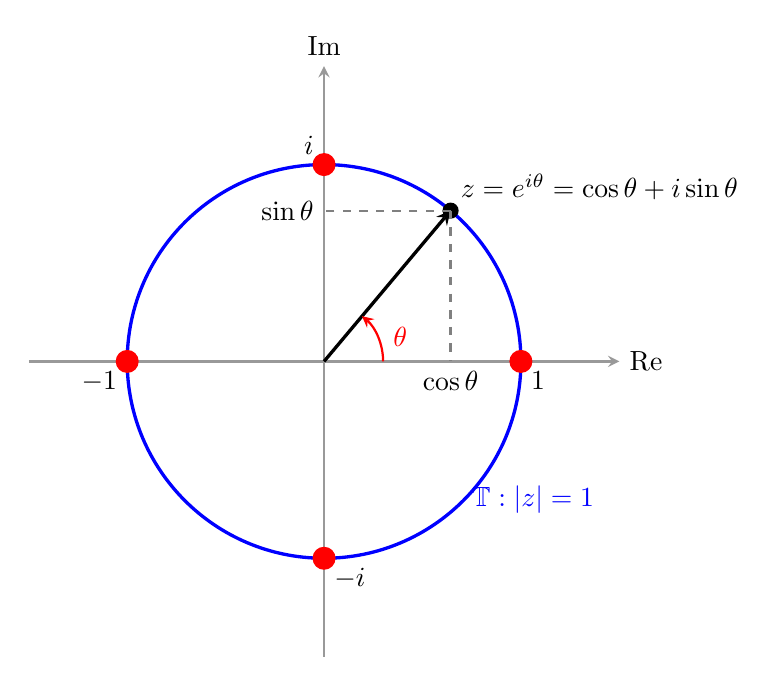
\begin{tikzpicture}[scale=2.5, thick, >=stealth]
        
        % x축과 y축 그리기 (Real and Imaginary axes)
        \draw[->, gray!80] (-1.5, 0) -- (1.5, 0) node[right, text=black] {$\text{Re}$};
        \draw[->, gray!80] (0, -1.5) -- (0, 1.5) node[above, text=black] {$\text{Im}$};
        
        % 반지름이 1인 단위원 (Unit Circle)
        \draw[blue, very thick] (0,0) circle (1);
        \node[blue, right] at (0.7, -0.7) {$\mathbb{T} : |z|=1$};
        
        % 임의의 점 e^{i\theta} 를 가리키는 벡터
        \def\angle{50} % 각도 설정 (50도)
        \draw[->, very thick] (0,0) -- (\angle:1);
        
        % e^{i\theta} 점 표시 및 라벨
        \filldraw[black] (\angle:1) circle (1pt) node[above right] {$z = e^{i\theta} = \cos\theta + i\sin\theta$};
        
        % 각도 \theta 표시 (arc 활용)
        \draw[->, red, thick] (0.3, 0) arc (0:\angle:0.3) node[midway, right, xshift=2pt] {$\theta$};
        
        % 삼각함수 성분을 보여주는 점선 (Projection lines)
        \draw[dashed, gray] (\angle:1) -- ({cos(\angle)}, 0) node[below, text=black] {$\cos\theta$};
        \draw[dashed, gray] (\angle:1) -- (0, {sin(\angle)}) node[left, text=black] {$\sin\theta$};
        
        % 텍스트에서 언급된 4제곱근 (4th roots of unity) 붉은 점 표시
        \filldraw[red] (1,0) circle (1.5pt) node[below right, text=black] {$1$};
        \filldraw[red] (0,1) circle (1.5pt) node[above left, text=black] {$i$};
        \filldraw[red] (-1,0) circle (1.5pt) node[below left, text=black] {$-1$};
        \filldraw[red] (0,-1) circle (1.5pt) node[below right, text=black] {$-i$};
        
    \end{tikzpicture}
    \caption{Geometric representation of the circle group $\mathbb{T}$ in the complex plane. Any element $z \in \mathbb{T}$ can be uniquely identified by the angle $\theta$ using Euler's formula \cite{dummit}. The red dots visually highlight the 4th roots of unity, which form a cyclic subgroup of order 4 \cite{gallian}.}
    \label{fig:circle_group}
\end{figure}

Within this circle group $\mathbb{T}$, the subset of complex numbers satisfying the polynomial equation $z^n = 1$ are called the $n$-th roots of unity \cite{dummit}. They form a finite cyclic subgroup of order $n$, strictly generated by the element $e^{i\frac{2\pi}{n}}$. 
For instance, the 4th roots of unity ($n=4$) are explicitly $\{1, i, -1, -i\}$, visually highlighted as the red dots in Figure \ref{fig:circle_group}, and they form a finite cyclic subgroup of order 4 \cite{gallian}.
\end{example}



\section{Permutation Groups}

\subsection{Definition and The Symmetric Group}

Permutation groups provide a highly concrete and fundamental way to construct and analyze finite groups through the concept of bijective mappings \cite{fraleigh}.

\begin{definition}[Permutation and Symmetric Group]
A permutation of a set $X$ is defined as a bijective function (one-to-one and onto) from $X$ to itself, mapping $X \rightarrow X$ \cite{dummit}. 
The set of all possible permutations of $X$, denoted by $S_X$, forms a group under the binary operation of function composition. If the set $X$ is finite and consists of $n$ elements, typically $X = \{1, 2, \dots, n\}$, this group is denoted as $S_n$ and is called the \emph{symmetric group on $n$ letters} \cite{gallian}.
\end{definition}

\begin{theorem}
The symmetric group $S_n$ is a valid group, and its order is $|S_n| = n!$ \cite{fraleigh}.
\end{theorem}

\begin{proof}
To verify that $S_n$ is a group, we check the group axioms:
\begin{enumerate}
    \item \emph{Identity:} The identity mapping $e: X \rightarrow X$ defined by $e(k) = k$ for all $k \in X$ is a bijection, thus $e \in S_n$ \cite{dummit}.
    \item \emph{Inverses:} If $f: X \rightarrow X$ is a bijection, its inverse function $f^{-1}: X \rightarrow X$ mathematically exists and is also a bijection. Therefore, every permutation has an inverse in $S_n$ \cite{fraleigh}.
    \item \emph{Closure and Associativity:} The composition of any two bijections $f, g: X \rightarrow X$ is strictly bijective. Function composition is inherently associative (i.e., $(f \circ g) \circ h = f \circ (g \circ h)$) \cite{gallian}.
\end{enumerate}
Since there are exactly $n$ choices for where to map the first element, $n-1$ for the second, and so forth, the total number of distinct bijective mappings is $n \times (n-1) \times \dots \times 1 = n!$. Hence, $|S_n| = n!$ \cite{dummit}.
\end{proof}

\begin{remark}
Any subgroup of $S_n$ is generically referred to as a \emph{permutation group} \cite{gallian}.
\end{remark}

\subsection{Two-Line Notation and Computations}

Permutations are frequently expressed using a two-line matrix notation, where the top row lists the elements of the domain, and the bottom row lists their corresponding images \cite{dummit}. For instance, a permutation $f \in S_3$ where $f(1)=2$, $f(2)=1$, and $f(3)=3$ is written as:
\begin{equation}
    f = \begin{pmatrix} 1 & 2 & 3 \\ 2 & 1 & 3 \end{pmatrix}
\end{equation}

\begin{example}[An Abelian Subgroup of $S_5$]
Consider a subgroup $G$ of the symmetric group $S_5$ consisting of the identity $id$ and the following three specific permutations \cite{dummit}:
\begin{equation}
    \sigma = \begin{pmatrix} 1 & 2 & 3 & 4 & 5 \\ 1 & 2 & 3 & 5 & 4 \end{pmatrix}, \quad 
    \tau = \begin{pmatrix} 1 & 2 & 3 & 4 & 5 \\ 3 & 2 & 1 & 4 & 5 \end{pmatrix}, \quad 
    \mu = \begin{pmatrix} 1 & 2 & 3 & 4 & 5 \\ 3 & 2 & 1 & 5 & 4 \end{pmatrix}
\end{equation}

By computing all possible compositions of these elements (for instance, evaluating $\sigma \cdot \tau = \mu$ and $\tau \cdot \sigma = \mu$ from right to left), we can construct the complete Cayley table for this subgroup $G$ \cite{fraleigh}:

\begin{table}[H]
    \centering
    \renewcommand{\arraystretch}{1.5} % 표의 세로 여백을 넓혀 가독성을 높입니다.
    \setlength{\tabcolsep}{10pt} % 표의 가로 여백을 넓힙니다.
    \begin{tabular}{c|cccc}
        $\circ$ & $id$ & $\sigma$ & $\tau$ & $\mu$ \\
        \hline
        $id$ & $id$ & $\sigma$ & $\tau$ & $\mu$ \\
        $\sigma$ & $\sigma$ & $id$ & $\mu$ & $\tau$ \\
        $\tau$ & $\tau$ & $\mu$ & $id$ & $\sigma$ \\
        $\mu$ & $\mu$ & $\tau$ & $\sigma$ & $id$ \\
    \end{tabular}
    \caption{The Cayley table for the subgroup $G = \{id, \sigma, \tau, \mu\}$.}
    \label{tab:cayley_S5_subgroup}
\end{table}

A careful observation of Table \ref{tab:cayley_S5_subgroup} reveals two critical algebraic properties:
\begin{enumerate}
    \item Every element is its own inverse, meaning $x \cdot x = id$ for all $x \in G$.
    \item The table is perfectly symmetric strictly across its main diagonal. This geometric symmetry formally guarantees that $x \cdot y = y \cdot x$ for all $x, y \in G$.
\end{enumerate}
Therefore, despite being a subgroup of the highly non-commutative group $S_5$, this specific subgroup $G$ is strictly commutative (abelian) \cite{gallian}. Structurally, this group is isomorphic to the Klein four-group ($V_4$).
\end{example}


\begin{example}[Non-commutativity of $S_n$]
Generally, for $n \ge 3$, the symmetric group $S_n$ is non-abelian \cite{fraleigh}. Consider two permutations $\sigma, \tau \in S_4$:
\begin{equation}
    \sigma = \begin{pmatrix} 1 & 2 & 3 & 4 \\ 4 & 1 & 2 & 3 \end{pmatrix}, \quad 
    \tau = \begin{pmatrix} 1 & 2 & 3 & 4 \\ 2 & 1 & 4 & 3 \end{pmatrix}
\end{equation}
We compute the composition $\sigma \cdot \tau$ by evaluating right-to-left (applying $\tau$ first, then $\sigma$) \cite{dummit}:
\begin{equation}
    \sigma \cdot \tau = \begin{pmatrix} 1 & 2 & 3 & 4 \\ 4 & 1 & 2 & 3 \end{pmatrix} \begin{pmatrix} 1 & 2 & 3 & 4 \\ 2 & 1 & 4 & 3 \end{pmatrix} = \begin{pmatrix} 1 & 2 & 3 & 4 \\ 1 & 4 & 3 & 2 \end{pmatrix}
\end{equation}
Conversely, computing $\tau \cdot \sigma$ yields a different outcome:
\begin{equation}
    \tau \cdot \sigma = \begin{pmatrix} 1 & 2 & 3 & 4 \\ 2 & 1 & 4 & 3 \end{pmatrix} \begin{pmatrix} 1 & 2 & 3 & 4 \\ 4 & 1 & 2 & 3 \end{pmatrix} = \begin{pmatrix} 1 & 2 & 3 & 4 \\ 3 & 2 & 1 & 4 \end{pmatrix}
\end{equation}
Since $\sigma \cdot \tau \neq \tau \cdot \sigma$, the group operation is strictly non-commutative \cite{gallian}.
\end{example}

\subsection{Cycle Notation}

\begin{definition}[Cycle of Length $k$]
A permutation $\sigma \in S_X$ is called a cycle of length $k$ (or a $k$-cycle) if there exist $k$ distinct elements $a_1, a_2, \dots, a_k \in X$ such that \cite{dummit}:
\begin{equation}
    \sigma(a_1) = a_2, \quad \sigma(a_2) = a_3, \quad \dots, \quad \sigma(a_k) = a_1
\end{equation}
and $\sigma(x) = x$ for all other elements $x \in X$ not in this set. We compactly denote this as $\sigma = (a_1 \; a_2 \; \dots \; a_k)$.
\end{definition}

\begin{example}[A 6-Cycle in $S_7$]
Consider the following permutation in $S_7$:
\begin{equation}
    \sigma = \begin{pmatrix} 1 & 2 & 3 & 4 & 5 & 6 & 7 \\ 6 & 3 & 5 & 1 & 4 & 2 & 7 \end{pmatrix}
\end{equation}
Tracing the mappings, we observe $1 \mapsto 6 \mapsto 2 \mapsto 3 \mapsto 5 \mapsto 4 \mapsto 1$, while $7$ remains strictly fixed \cite{gallian}. This forms a cycle of length 6, written as $\sigma = (1 \; 6 \; 2 \; 3 \; 5 \; 4)$.

% --- TikZ: 순환 표기법의 시각적 매핑 ---
\begin{figure}[H]
    \centering
    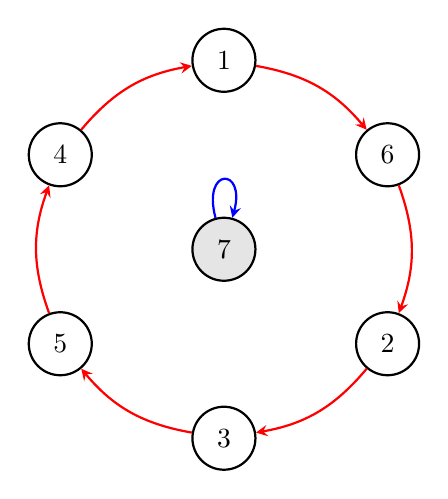
\begin{tikzpicture}[scale=1.2, >=stealth, thick]
        % 원형으로 노드 배치
        \node[circle, draw, minimum size=0.8cm] (n1) at (90:2) {1};
        \node[circle, draw, minimum size=0.8cm] (n6) at (30:2) {6};
        \node[circle, draw, minimum size=0.8cm] (n2) at (330:2) {2};
        \node[circle, draw, minimum size=0.8cm] (n3) at (270:2) {3};
        \node[circle, draw, minimum size=0.8cm] (n5) at (210:2) {5};
        \node[circle, draw, minimum size=0.8cm] (n4) at (150:2) {4};
        
        % 고정점 7 노드 배치
        \node[circle, draw, fill=gray!20, minimum size=0.8cm] (n7) at (0,0) {7};
        \draw[->, loop above, blue] (n7) to (n7);

        % 순환 화살표 그리기
        \draw[->, red] (n1) edge[bend left=20] (n6);
        \draw[->, red] (n6) edge[bend left=20] (n2);
        \draw[->, red] (n2) edge[bend left=20] (n3);
        \draw[->, red] (n3) edge[bend left=20] (n5);
        \draw[->, red] (n5) edge[bend left=20] (n4);
        \draw[->, red] (n4) edge[bend left=20] (n1);
        
    \end{tikzpicture}
    \caption{Visual representation of the 6-cycle $\sigma = (1 \; 6 \; 2 \; 3 \; 5 \; 4)$ in $S_7$. The element $7$ is fixed, mapping back to itself \cite{dummit}.}
\end{figure}
\end{example}

\begin{example}[Disjoint Cycles Decomposition]
Not every permutation is a single cycle \cite{fraleigh}. However, every permutation can be uniquely expressed as a product of disjoint cycles. Consider:
\begin{equation}
    \begin{pmatrix} 1 & 2 & 3 & 4 & 5 & 6 \\ 2 & 4 & 1 & 3 & 6 & 5 \end{pmatrix} = (1 \; 2 \; 4 \; 3)(5 \; 6)
\end{equation}
Here, the domain structurally splits into two independent non-overlapping subsets: one subset cycles through $\{1, 2, 4, 3\}$ and the other merely swaps $\{5, 6\}$ \cite{gallian}.
\end{example}

\begin{proposition}[Disjoint Cycles Commute]
Let $\sigma$ and $\tau$ be disjoint cycles in $S_X$. Then they strictly commute, meaning $\sigma \tau = \tau \sigma$ \cite{fraleigh}.
\end{proposition}

\begin{proof}
Let $A$ be the set of elements moved by $\sigma$ (e.g., $A = \{a_1, \dots, a_k\}$), and let $B$ be the set of elements moved by $\tau$ (e.g., $B = \{b_1, \dots, b_l\}$) \cite{dummit}. Because $\sigma$ and $\tau$ are disjoint cycles, their respective sets of moved elements are entirely disjoint, implying $A \cap B = \emptyset$ \cite{gallian}.

To formally prove $\sigma(\tau(x)) = \tau(\sigma(x))$ for all $x \in X$, we evaluate three distinct cases \cite{dummit}:
\begin{enumerate}
    \item If $x \notin A \cup B$, then both cycles fix $x$. Thus, $\sigma(\tau(x)) = \sigma(x) = x$ and $\tau(\sigma(x)) = \tau(x) = x$.
    \item If $x \in A$, then $x \notin B$. Since $\sigma(x)$ is also contained in $A$, it follows that $\sigma(x) \notin B$. Therefore, the cycle $\tau$ acts as the identity on both $x$ and $\sigma(x)$. We get $\tau(\sigma(x)) = \sigma(x)$, and $\sigma(\tau(x)) = \sigma(x)$.
    \item If $x \in B$, by symmetric logic, $x \notin A$ and $\tau(x) \notin A$. Thus, $\sigma(\tau(x)) = \tau(x)$ and $\tau(\sigma(x)) = \tau(x)$.
\end{enumerate}
Since the mappings are identical in all possible cases, the group operation commutes, meaning $\sigma \tau = \tau \sigma$ \cite{fraleigh}.
\end{proof}

% --- TikZ: 서로소인 순환의 교환법칙 시각화 ---
\begin{figure}[H]
    \centering
    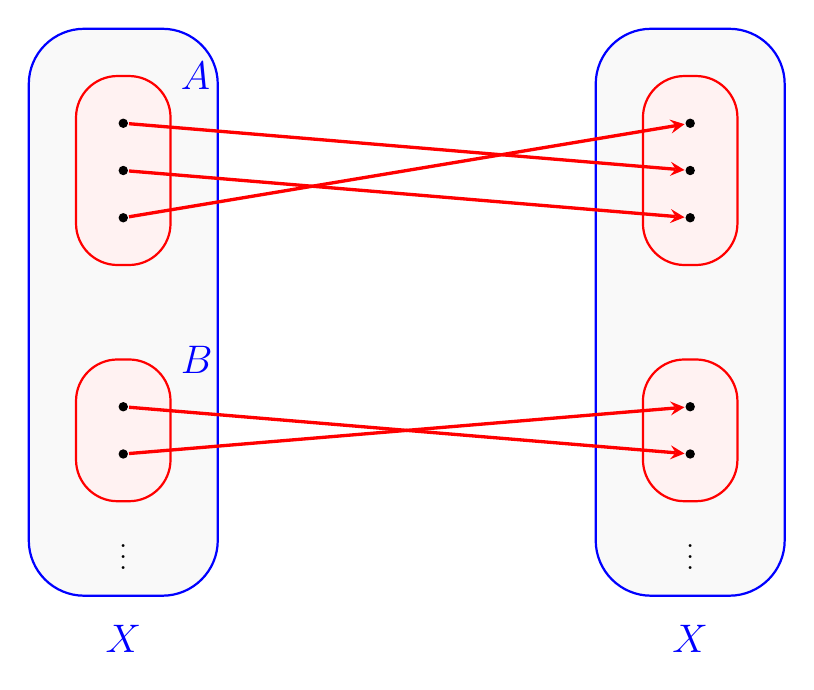
\begin{tikzpicture}[scale=1.2, thick, >=stealth]
        % 왼쪽 정의역 X 타원
        \draw[blue, rounded corners=20pt, fill=gray!5] (-1.5, 3) rectangle (0.5, -3);
        \node[below, blue, font=\Large] at (-0.5, -3.2) {$X$};

        % 오른쪽 공역 X 타원
        \draw[blue, rounded corners=20pt, fill=gray!5] (4.5, 3) rectangle (6.5, -3);
        \node[below, blue, font=\Large] at (5.5, -3.2) {$X$};

        % 왼쪽 부분집합 A, B (붉은 테두리)
        \draw[red, rounded corners=15pt, fill=red!5] (-1, 2.5) rectangle (0, 0.5);
        \node[right, blue, font=\Large] at (0, 2.5) {$A$};
        
        \draw[red, rounded corners=15pt, fill=red!5] (-1, -0.5) rectangle (0, -2);
        \node[right, blue, font=\Large] at (0, -0.5) {$B$};

        % 오른쪽 부분집합 A, B (붉은 테두리)
        \draw[red, rounded corners=15pt, fill=red!5] (5, 2.5) rectangle (6, 0.5);
        \draw[red, rounded corners=15pt, fill=red!5] (5, -0.5) rectangle (6, -2);

        % 집합 A 내부의 원소(노드)들
        \node[circle, fill=black, inner sep=1.2pt] (a1L) at (-0.5, 2) {};
        \node[circle, fill=black, inner sep=1.2pt] (a2L) at (-0.5, 1.5) {};
        \node[circle, fill=black, inner sep=1.2pt] (a3L) at (-0.5, 1) {};

        \node[circle, fill=black, inner sep=1.2pt] (a1R) at (5.5, 2) {};
        \node[circle, fill=black, inner sep=1.2pt] (a2R) at (5.5, 1.5) {};
        \node[circle, fill=black, inner sep=1.2pt] (a3R) at (5.5, 1) {};

        % 집합 B 내부의 원소(노드)들
        \node[circle, fill=black, inner sep=1.2pt] (b1L) at (-0.5, -1) {};
        \node[circle, fill=black, inner sep=1.2pt] (b2L) at (-0.5, -1.5) {};

        \node[circle, fill=black, inner sep=1.2pt] (b1R) at (5.5, -1) {};
        \node[circle, fill=black, inner sep=1.2pt] (b2R) at (5.5, -1.5) {};

        % 고정된 나머지 원소들 표시 (점선)
        \node at (-0.5, -2.5) {$\vdots$};
        \node at (5.5, -2.5) {$\vdots$};

        % 집합 A 내부에서의 맵핑 (붉은 화살표 크로스)
        \draw[->, red, very thick] (a1L) -- (a2R);
        \draw[->, red, very thick] (a2L) -- (a3R);
        \draw[->, red, very thick] (a3L) -- (a1R);

        % 집합 B 내부에서의 맵핑 (붉은 화살표 크로스)
        \draw[->, red, very thick] (b1L) -- (b2R);
        \draw[->, red, very thick] (b2L) -- (b1R);

    \end{tikzpicture}
    \caption{A bipartite mapping diagram illustrating that disjoint cycles operate on completely independent subsets $A$ and $B$. Because $A \cap B = \emptyset$, their respective mappings do not interfere with each other, visually confirming the algebraic property $\sigma \tau = \tau \sigma$ \cite{gallian}.}
    \label{fig:disjoint_cycles}
\end{figure}


\subsection{Transpositions and the Parity of Permutations}

\begin{definition}[Transposition]
A cycle of length 2, denoted as $(a \; b) \in S_X$, is called a transposition \cite{fraleigh}. It effectively swaps the elements $a$ and $b$ while leaving all other elements in $X$ strictly fixed. A fundamental property of any transposition is that it is its own inverse, meaning $(a \; b) = (b \; a)$ and $(a \; b)^{-1} = (a \; b)$ \cite{dummit}.
\end{definition}

% --- TikZ: 호환(Transposition)의 이분 그래프(Bipartite Graph) 매핑 시각화 ---
\begin{figure}[H]
    \centering
    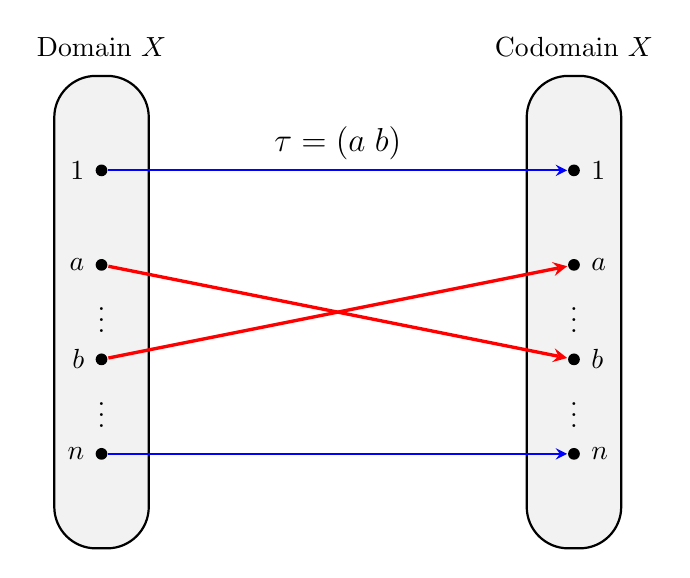
\begin{tikzpicture}[scale=1.2, thick, >=stealth]
        % 왼쪽 도메인 타원
        \draw[fill=gray!10, rounded corners=15pt] (-1, 2.5) rectangle (0, -2.5);
        \node[above] at (-0.5, 2.6) {Domain $X$};
        
        % 오른쪽 공역 타원
        \draw[fill=gray!10, rounded corners=15pt] (4, 2.5) rectangle (5, -2.5);
        \node[above] at (4.5, 2.6) {Codomain $X$};
        
        % 노드 정의 (Domain)
        \node[circle, fill=black, inner sep=1.5pt, label=left:{$1$}] (L1) at (-0.5, 1.5) {};
        \node[circle, fill=black, inner sep=1.5pt, label=left:{$a$}] (La) at (-0.5, 0.5) {};
        \node[circle, fill=black, inner sep=1.5pt, label=left:{$b$}] (Lb) at (-0.5, -0.5) {};
        \node[circle, fill=black, inner sep=1.5pt, label=left:{$n$}] (Ln) at (-0.5, -1.5) {};
        \node at (-0.5, 0) {$\vdots$};
        \node at (-0.5, -1) {$\vdots$};

        % 노드 정의 (Codomain)
        \node[circle, fill=black, inner sep=1.5pt, label=right:{$1$}] (R1) at (4.5, 1.5) {};
        \node[circle, fill=black, inner sep=1.5pt, label=right:{$a$}] (Ra) at (4.5, 0.5) {};
        \node[circle, fill=black, inner sep=1.5pt, label=right:{$b$}] (Rb) at (4.5, -0.5) {};
        \node[circle, fill=black, inner sep=1.5pt, label=right:{$n$}] (Rn) at (4.5, -1.5) {};
        \node at (4.5, 0) {$\vdots$};
        \node at (4.5, -1) {$\vdots$};
        
        % 매핑 화살표 (Transposition (a b))
        \draw[->, blue] (L1) -- (R1);
        \draw[->, red, very thick] (La) -- (Rb);
        \draw[->, red, very thick] (Lb) -- (Ra);
        \draw[->, blue] (Ln) -- (Rn);
        
        \node[above, font=\large] at (2, 1.5) {$\tau = (a \; b)$};
    \end{tikzpicture}
    \caption{A bipartite mapping diagram illustrating the transposition $\tau = (a \; b)$. The elements $a$ and $b$ are strictly swapped (red arrows), while all other elements map directly to themselves (blue arrows) \cite{gallian}.}
\end{figure}

\begin{proposition}[Decomposition into Transpositions]
Any permutation on a set containing at least two elements can be expressed as a finite product (composition) of transpositions \cite{fraleigh}. 
\end{proposition}

\begin{proof}
Since every permutation can be written as a product of disjoint cycles, it suffices to show that any single cycle can be decomposed into transpositions \cite{dummit}. A cycle of length $k$ can be systematically decomposed as:
\begin{equation} \label{eq:cycle_decomp}
    (a_1 \; a_2 \; \dots \; a_k) = (a_1 \; a_k)(a_1 \; a_{k-1}) \dots (a_1 \; a_3)(a_1 \; a_2)
\end{equation}
By applying the transpositions from right to left, we observe that $a_1 \mapsto a_2$, $a_2 \mapsto a_3$, and so forth, exactly reproducing the original cycle. Since every cycle can be factored this way, the proposition holds \cite{gallian}.
\end{proof}

\begin{remark}
The decomposition into transpositions is not unique. For example, the identity permutation can be written as $id = (1 \; 2)(1 \; 2)$ or $id = (2 \; 3)(1 \; 4)(1 \; 4)(2 \; 3)$. However, the \emph{parity} (even or oddness) of the number of transpositions is always invariant \cite{dummit}.
\end{remark}

\begin{lemma}[Parity of the Identity]
If the identity permutation is written as a product of transpositions, $id = \tau_1 \tau_2 \dots \tau_r$, then the number of transpositions $r$ must strictly be an even number \cite{gallian}.
\end{lemma}

\begin{definition}[Sign and Parity of a Permutation]
The sign (or signature/parity) of a permutation $\sigma \in S_n$, denoted as $\operatorname{sgn}(\sigma)$, is defined mathematically by the number of transpositions $r$ required to express it:
\begin{equation}
    \operatorname{sgn}(\sigma) = (-1)^r
\end{equation}
If $\operatorname{sgn}(\sigma) = 1$ (meaning $r$ is even), we say $\sigma$ is an \emph{even permutation}. If $\operatorname{sgn}(\sigma) = -1$ (meaning $r$ is odd), we say $\sigma$ is an \emph{odd permutation} \cite{fraleigh}. The well-definedness of this map $\operatorname{sgn}: S_n \to \{-1, 1\}$ is guaranteed by the preceding lemma \cite{dummit}.
\end{definition}

\begin{lemma}[Multiplicativity of the Sign]
For any two permutations $\sigma, \sigma' \in S_n$, the sign function is strictly multiplicative:
\begin{equation}
    \operatorname{sgn}(\sigma \sigma') = \operatorname{sgn}(\sigma) \operatorname{sgn}(\sigma')
\end{equation}
\end{lemma}

\begin{proof}
Let $\sigma$ and $\sigma'$ be expressed as products of transpositions:
\begin{equation}
    \sigma = \tau_1 \tau_2 \dots \tau_r \quad \text{and} \quad \sigma' = \tau'_1 \tau'_2 \dots \tau'_s
\end{equation}
The composition $\sigma \sigma'$ is simply the concatenated product of these transpositions:
\begin{equation}
    \sigma \sigma' = \tau_1 \dots \tau_r \tau'_1 \dots \tau'_s
\end{equation}
This combined expression consists of exactly $r + s$ transpositions \cite{dummit}. By the definition of the sign function, we can compute:
\begin{equation}
    \operatorname{sgn}(\sigma \sigma') = (-1)^{r+s} = (-1)^r (-1)^s = \operatorname{sgn}(\sigma) \operatorname{sgn}(\sigma')
\end{equation}
This confirms that composing two even (or two odd) permutations yields an even permutation, while composing an even and an odd permutation yields an odd permutation \cite{gallian}.
\end{proof}


\subsection{The Alternating Group and the Dihedral Group}

\begin{definition}[The Alternating Group]
For any integer $n \ge 2$, the alternating group of degree $n$, denoted by $A_n$, is defined as the set of all even permutations within the symmetric group $S_n$ \cite{dummit}.
\end{definition}

\begin{theorem}
The set of even permutations $A_n$ forms a valid subgroup of the symmetric group $S_n$ \cite{fraleigh}.
\end{theorem}

\begin{proof}
We can formally prove this by verifying the standard subgroup criteria.
\begin{enumerate}
    \item \emph{Identity:} The identity permutation $id$ has $\operatorname{sgn}(id) = 1$, which strictly implies $id \in A_n$ \cite{dummit}.
    \item \emph{Closure:} Let $\sigma, \sigma' \in A_n$. Since $\operatorname{sgn}(\sigma) = 1$ and $\operatorname{sgn}(\sigma') = 1$, their composition yields $\operatorname{sgn}(\sigma\sigma') = \operatorname{sgn}(\sigma)\operatorname{sgn}(\sigma') = 1$. Thus, $\sigma\sigma' \in A_n$ \cite{fraleigh}.
    \item \emph{Inverses:} For any $\sigma \in A_n$, $\operatorname{sgn}(\sigma\sigma^{-1}) = \operatorname{sgn}(id) = 1$. Since $\operatorname{sgn}(\sigma) = 1$, it algebraically forces $\operatorname{sgn}(\sigma^{-1}) = 1$, meaning $\sigma^{-1} \in A_n$ \cite{gallian}.
\end{enumerate}
Therefore, $A_n \leq S_n$.
\end{proof}

\begin{theorem}[Order of the Alternating Group]
The order of the alternating group $A_n$ is exactly half the order of the symmetric group $S_n$, explicitly $|A_n| = \frac{n!}{2}$ \cite{gallian}.
\end{theorem}

\begin{proof}
Let $B_n$ be the set of all odd permutations in $S_n$. We construct a strict bijective mapping between $A_n$ and $B_n$. Fix an arbitrary transposition $\tau \in S_n$. Define a mapping $f: A_n \to B_n$ by $f(\sigma) = \tau \sigma$. 
Since $\sigma$ is an even permutation, composing it with one transposition $\tau$ changes its parity, ensuring the result is an odd permutation \cite{dummit}.

This mapping is injective because $\tau\sigma = \tau\sigma'$ implies $\sigma = \sigma'$ by left cancellation. It is surjective because any odd permutation $\mu \in B_n$ can be written as $\tau(\tau\mu)$, where $\tau\mu \in A_n$. 
Since $f$ is a perfect bijection, $|A_n| = |B_n|$. Because $S_n = A_n \cup B_n$ is a disjoint union, $2|A_n| = |S_n| = n!$, which concludes the proof \cite{fraleigh}.
\end{proof}


\subsection{The Dihedral Group}

\begin{definition}[The Dihedral Group]
The $n$-th dihedral group $D_n$ is defined as the group of isometries leaving a regular $n$-gon strictly invariant. These isometries inherently consist of spatial rotations and reflections \cite{gallian}.
\end{definition}

% --- TikZ: 5-gon (정오각형) 대칭군 시각화 ---
\begin{figure}[H]
    \centering
    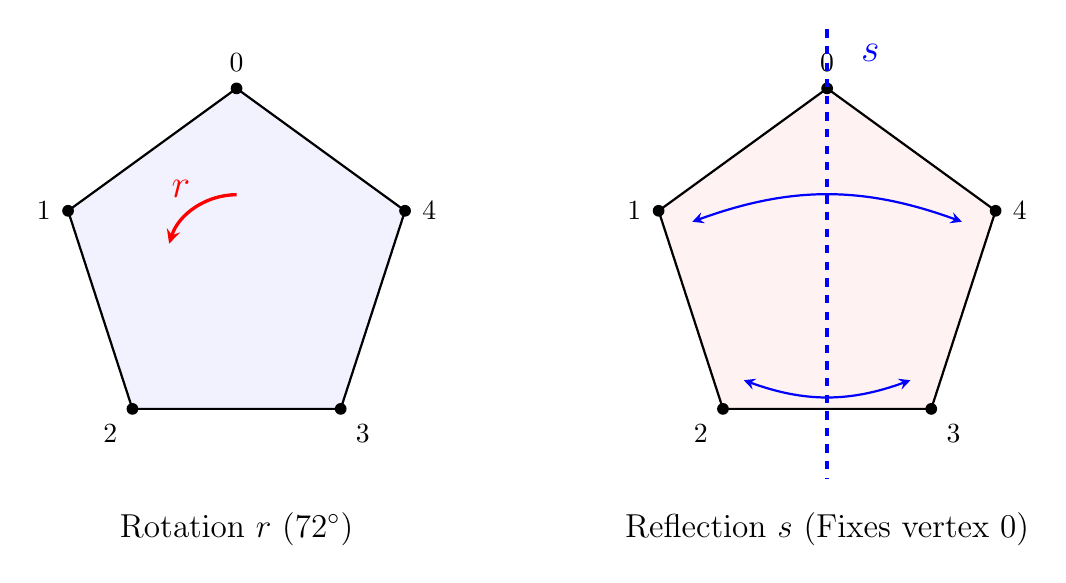
\begin{tikzpicture}[scale=1.5, thick, >=stealth]
        
        % ==========================================
        % 1. Rotation r (회전 변환)
        % ==========================================
        \begin{scope}[xshift=0cm]
            % 정오각형 그리기 (반지름 1.5, 꼭짓점 각도: 90, 162, 234, 306, 18)
            \draw[fill=blue!5] (90:1.5) -- (162:1.5) -- (234:1.5) -- (306:1.5) -- (18:1.5) -- cycle;
            
            % 꼭짓점과 라벨 (노드)
            \node[circle, fill=black, inner sep=1.5pt, label=above:{$0$}] (v0) at (90:1.5) {};
            \node[circle, fill=black, inner sep=1.5pt, label=left:{$1$}] (v1) at (162:1.5) {};
            \node[circle, fill=black, inner sep=1.5pt, label=below left:{$2$}] (v2) at (234:1.5) {};
            \node[circle, fill=black, inner sep=1.5pt, label=below right:{$3$}] (v3) at (306:1.5) {};
            \node[circle, fill=black, inner sep=1.5pt, label=right:{$4$}] (v4) at (18:1.5) {};
            
            % 회전을 나타내는 화살표 (중앙에 원호 배치)
            \draw[->, red, very thick] (90:0.6) arc (90:162:0.6);
            \node[red, font=\Large] at (126:0.8) {$r$};
            
            % 하단 설명
            \node[below, font=\large] at (0, -2) {Rotation $r$ ($72^\circ$)};
        \end{scope}
        
        % ==========================================
        % 2. Reflection s (반사 변환)
        % ==========================================
        \begin{scope}[xshift=5cm]
            % 정오각형 그리기
            \draw[fill=red!5] (90:1.5) -- (162:1.5) -- (234:1.5) -- (306:1.5) -- (18:1.5) -- cycle;
            
            % 꼭짓점과 라벨
            \node[circle, fill=black, inner sep=1.5pt, label=above:{$0$}] (v0) at (90:1.5) {};
            \node[circle, fill=black, inner sep=1.5pt, label=left:{$1$}] (v1) at (162:1.5) {};
            \node[circle, fill=black, inner sep=1.5pt, label=below left:{$2$}] (v2) at (234:1.5) {};
            \node[circle, fill=black, inner sep=1.5pt, label=below right:{$3$}] (v3) at (306:1.5) {};
            \node[circle, fill=black, inner sep=1.5pt, label=right:{$4$}] (v4) at (18:1.5) {};
            
            % 꼭짓점 0을 지나는 수직 반사축 (점선)
            \draw[dashed, blue, very thick] (0, 2) -- (0, -1.8);
            
            % 원소가 스왑(Swap) 됨을 보여주는 교환 화살표
            \draw[<->, blue, thick] (162:1.2) to[bend left=20] (18:1.2);
            \draw[<->, blue, thick] (234:1.2) to[bend right=20] (306:1.2);
            
            % 기호 표시
            \node[blue, font=\Large, right] at (0.2, 1.8) {$s$};
            
            % 하단 설명
            \node[below, font=\large] at (0, -2) {Reflection $s$ (Fixes vertex $0$)};
        \end{scope}
        
    \end{tikzpicture}
    \caption{Consider the dihedral group $D_5$, which algebraically represents the symmetries of a regular pentagon. The order of $D_5$ is precisely $2 \times 5 = 10$. Let the 5 vertices be labeled $0, 1, 2, 3, 4$ in counterclockwise order. The fundamental rotation $r$ shifts each vertex counterclockwise by exactly $72^\circ$ ($2\pi/5$). The fundamental reflection $s$ geometrically fixes vertex $0$ and symmetrically swaps the remaining vertices (e.g., $1 \leftrightarrow 4$ and $2 \leftrightarrow 3$) strictly across the vertical axis of symmetry \cite{gallian}.}
    \label{fig:D5_5gon}
\end{figure}


\begin{theorem}[Order of $D_n$]
The dihedral group $D_n$ is a subgroup of the symmetric group $S_n$, and it consists of exactly $2n$ elements \cite{dummit}.
\end{theorem}

\begin{proof}
By tracking the permutations of the $n$ distinct vertices of the regular $n$-gon, we can naturally embed $D_n$ into $S_n$ \cite{fraleigh}. 
First, there are exactly $n$ distinct rotational symmetries, which cyclically permute the vertices (e.g., mapping vertex $1 \mapsto k$, $2 \mapsto k+1$, and so on up to $n$). 
Additionally, there are exactly $n$ distinct symmetries involving a reflection (or a reflection followed by a rotation), which reverse the sequential orientation of the vertices (e.g., mapping $1 \mapsto k$, $2 \mapsto k-1$). 
Summing these two disjoint sets of isometries yields exactly $n + n = 2n$ elements \cite{gallian}. Therefore, $|D_n| = 2n$.
\end{proof}

\begin{theorem}[Generators and Relations of $D_n$]
For $n \ge 3$, the dihedral group $D_n$ consists of all possible products of two fundamental elements $r$ and $s$, satisfying the following algebraic relations \cite{dummit}:
\begin{equation}
    r^n = id, \quad s^2 = id, \quad srs = r^{-1}
\end{equation}
\end{theorem}

\begin{proof}
Let $r$ denote a clockwise rotation by an angle of $\frac{2\pi}{n}$. Clearly, applying this rotation $n$ times returns the polygon to its exact original position, strictly implying $r^n = id$. The cyclic subgroup $\langle r \rangle$ contains all the $n$ purely rotational symmetries generated by $r$ \cite{fraleigh}.
    
Let $s$ denote a reflection that leaves at least one vertex strictly invariant. Applying a geometric reflection twice restores the original orientation, so clearly $s^2 = id$ \cite{gallian}. 
Since $D_n$ is generated entirely by rotations and reflections, all elements of $D_n$ can be expressed in the form $r^k s^l$, where the exponent $l \in \{0, 1\}$ \cite{dummit}.

% --- TikZ: 회전 r과 반사 s의 직관적 시각화 (노트 필기 완벽 반영) ---
\begin{figure}[H]
    \centering
    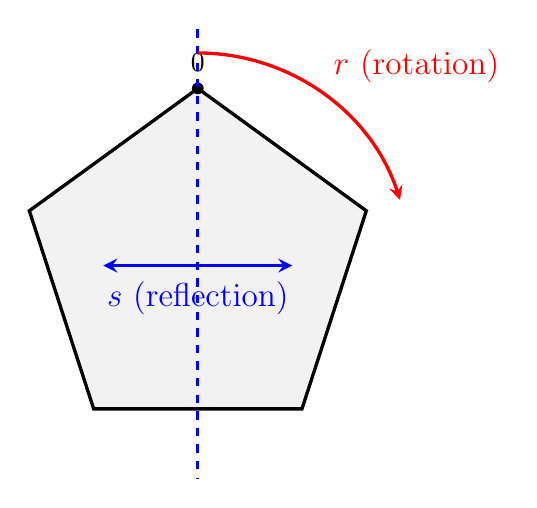
\begin{tikzpicture}[scale=1.5, thick, >=stealth]
        % 정n각형 그리기 (직관성을 위해 노트 필기와 동일하게 n=5인 정오각형 묘사)
        \draw[fill=gray!10, draw=black, very thick] (90:1.5) -- (18:1.5) -- (306:1.5) -- (234:1.5) -- (162:1.5) -- cycle;
        
        % 고정된 꼭짓점 0 (상단)
        \node[circle, fill=black, inner sep=1.5pt, label=above:{$0$}] (v0) at (90:1.5) {};
        
        % 수직 반사축 (Reflection s) - 꼭짓점 0을 지나는 점선
        \draw[dashed, blue, very thick] (0, 2) -- (0, -1.8);
        
        % 반사 s를 나타내는 좌우 화살표 (노트 필기의 중앙 <-> 형태 반영)
        \draw[<->, blue, very thick] (-0.8, 0) -- (0.8, 0) node[midway, below, yshift=-2pt, font=\large] {$s$ (reflection)};
        
        % 시계방향 회전 r을 나타내는 곡선 화살표 (노트 필기의 둥근 화살표 반영)
        \draw[->, red, very thick] (90:1.8) arc (90:18:1.8) node[midway, above right, font=\large] {$r$ (rotation)};
        
    \end{tikzpicture}
    \caption{Geometric visualization of the generators $r$ and $s$ on a regular polygon (illustrated here with $n=5$). The clockwise rotation $r$ shifts the vertices by $\frac{2\pi}{n}$, while the reflection $s$ mirrors the polygon across the axis of symmetry explicitly passing through vertex $0$ \cite{gallian}.}
    \label{fig:Dn_generators_combined}
\end{figure}

To rigorously prove the non-abelian relation $srs = r^{-1}$, let us label the vertices of the $n$-gon using the integers modulo $n$, forming the set $\mathbb{Z}_n$. Without loss of generality, let the vertex fixed by the reflection $s$ be labeled "$0$" \cite{gallian}. 
The mathematical actions of $r$ and $s$ on any arbitrary vertex $k \in \mathbb{Z}_n$ are formally defined as:
\begin{equation}
    r(k) = k + 1 \pmod n, \quad s(k) = -k \equiv n - k \pmod n
\end{equation}

We now systematically evaluate the composition $srsr$ acting on the vertex $k$ \cite{dummit}:
\begin{align}
    (srsr)(k) &= srs(k+1) \\
    &= sr(n - (k+1)) \\
    &= s(n - k - 1 + 1) \\
    &= s(n - k) \\
    &= n - (n - k) = k
\end{align}

Since the result is $(srsr)(k) = k$ for all possible vertices $k \in \mathbb{Z}_n$, the combined transformation acts completely identically to the identity mapping, meaning $srsr = id$ \cite{fraleigh}. Multiplying both sides of this equation by $r^{-1}$ on the right yields the final relation:
\begin{equation}
    srs = r^{-1}
\end{equation}
\cite{dummit}.
\end{proof}



\section{Symmetry Group of the Cube}

\begin{theorem}[Rotational Symmetries of a Cube]
The group of strictly rotational symmetries leaving a solid cube invariant is isomorphic to the symmetric group $S_4$ \cite{dummit}.
\end{theorem}

\begin{proof}
A cube intrinsically possesses exactly 4 main body diagonals connecting opposite vertices. Any spatial rotation of the cube uniquely and validly permutes these 4 distinct diagonals \cite{gallian}. 

To calculate the exact order of this rotational group $G$, observe that any of the 6 square faces can be chosen to face "upward." For each chosen top face, there are exactly 4 possible rotational orientations around the vertical axis \cite{fraleigh}. Thus, the total number of rotational symmetries is exactly $|G| = 6 \times 4 = 24$. Since $|S_4| = 4! = 24$, and every rotation induces a unique permutation of the diagonals, the group of rotations is isomorphic to $S_4$ \cite{dummit}.
\end{proof}

% --- TikZ: 정육면체의 4개 주대각선 시각화 ---
\begin{figure}[H]
    \centering
    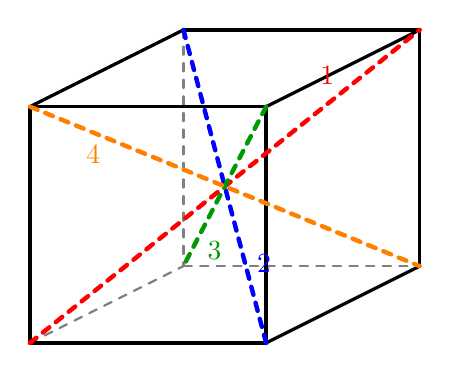
\begin{tikzpicture}[scale=1.5, thick, line join=round, line cap=round]
        % ---------------------------------------------------
        % 투영 각도(Viewing Angle) 조절을 위한 오프셋 변수
        % 이 값을 변경하면 정육면체의 기울기를 쉽게 조절할 수 있습니다.
        % ---------------------------------------------------
        \def\dx{1.3}
        \def\dy{0.65}
        
        % 뒷면 (Back face) 좌표 설정
        \coordinate (A') at (\dx, \dy);
        \coordinate (B') at (2+\dx, \dy);
        \coordinate (C') at (2+\dx, 2+\dy);
        \coordinate (D') at (\dx, 2+\dy);
        
        % 앞면 (Front face) 좌표 설정
        \coordinate (A) at (0, 0);
        \coordinate (B) at (2, 0);
        \coordinate (C) at (2, 2);
        \coordinate (D) at (0, 2);

        % 정육면체 모서리 그리기
        % 뒷면에 가려진 모서리는 회색 점선으로 처리하여 입체감을 극대화합니다.
        \draw[gray, dashed] (A') -- (B');
        \draw[black, very thick] (B') -- (C');
        \draw[black, very thick] (C') -- (D');
        \draw[gray, dashed] (D') -- (A');

        \draw[gray, dashed] (A) -- (A');
        \draw[black, very thick] (B) -- (B');
        \draw[black, very thick] (C) -- (C');
        \draw[black, very thick] (D) -- (D');
        
        % 앞면 테두리
        \draw[black, very thick] (A) -- (B) -- (C) -- (D) -- cycle;

        % 4개의 주대각선 (Main diagonals)
        % 겹침을 방지하기 위해 pos 속성을 사용하여 번호 라벨을 중심에서 바깥으로 밀어냅니다.
        \draw[red, ultra thick, dashed] (A) -- (C') node[pos=0.8, above left=-2pt] {1};
        \draw[blue, ultra thick, dashed] (B) -- (D') node[pos=0.2, above right=-2pt] {2};
        \draw[green!60!black, ultra thick, dashed] (C) -- (A') node[pos=0.8, below right=-2pt] {3};
        \draw[orange, ultra thick, dashed] (D) -- (B') node[pos=0.2, below left=-2pt] {4};
        
    \end{tikzpicture}
    \caption{The 4 main diagonals of a cube. Any 3D rotation of the cube corresponds to a valid permutation of these 4 distinct diagonals, geometrically demonstrating the isomorphism to $S_4$ \cite{gallian}.}
    \label{fig:cube_diagonals}
\end{figure}

\begin{remark}[The Full Symmetry Group of the Cube]
While the group of strictly rotational symmetries (orientation-preserving isometries) is isomorphic to $S_4$ with an order of 24, the \emph{full} symmetry group of the cube additionally includes reflections and the central inversion (orientation-reversing isometries) \cite{dummit}. 

Since the central inversion mathematically commutes with all possible geometric rotations in 3D space, the full symmetry group has exactly $24 \times 2 = 48$ elements. Algebraically, this full group is strictly isomorphic to the direct product $S_4 \times \mathbb{Z}_2$ \cite{gallian}. The rigorous mathematical proof of this structural isomorphism, along with a detailed analysis of the central inversion's role, will be thoroughly discussed in a later section.
\end{remark}

\section{Cosets and Lagrange's Theorem}

\subsection{Definition of Cosets}

\begin{definition}[Left and Right Cosets]
Let $H$ be a subgroup of a group $G$, and let $g \in G$. The \emph{left coset} of $H$ in $G$ containing $g$ is formally defined as the set \cite{fraleigh}:
\begin{equation}
    gH = \{gh \mid h \in H\}
\end{equation}
Similarly, the \emph{right coset} of $H$ in $G$ containing $g$ is defined as $Hg = \{hg \mid h \in H\}$ \cite{dummit}.
\end{definition}

\begin{example}[Cosets in $\mathbb{Z}_6$]
Let $G = \mathbb{Z}_6$ under addition, and consider the subgroup $H = \{0, 3\}$ \cite{gallian}. Because $G$ is an abelian group, the left and right cosets perfectly coincide ($g+H = H+g$). The distinct cosets are iteratively calculated as:
\begin{align}
    0 + H &= 3 + H = \{0, 3\} = H \\
    1 + H &= 4 + H = \{1, 4\} \\
    2 + H &= 5 + H = \{2, 5\}
\end{align}
\end{example}

\begin{example}[Equality of Left and Right Cosets]
Let $G = S_3$, and consider the subgroup $H = \{(1), (123), (132)\}$, which is the alternating group $A_3$. We evaluate the left and right cosets containing the specific element $(12)$ \cite{dummit}:
\begin{align}
    \text{Left Coset: } (12)H &= \{(12)(1), (12)(123), (12)(132)\} \\
    &= \{(12), (23), (13)\} \nonumber \\[5pt]
    \text{Right Coset: } H(12) &= \{(1)(12), (123)(12), (132)(12)\} \\
    &= \{(12), (13), (23)\} \nonumber
\end{align}
Since $(12)H = H(12)$ (and this holds true for any element in $G$), the left and right cosets perfectly coincide. Such a subgroup where left and right cosets are always equal is geometrically and algebraically symmetric, and is formally called a \emph{normal subgroup} \cite{gallian}.
\end{example}

\begin{example}[Non-equality of Left and Right Cosets]
Let $G = S_3$, and consider the non-normal subgroup $K = \{(1), (12)\}$. We rigorously evaluate all distinct left and right cosets by computing the disjoint cycle multiplications strictly from right to left \cite{fraleigh}:
\begin{align}
    \text{Left Cosets:} \nonumber \\
    (1)K = (12)K &= \{(1), (12)\} \\
    (13)K = (123)K &= \{(13)(1), (13)(12)\} = \{(13), (123)\} \\
    (23)K = (132)K &= \{(23)(1), (23)(12)\} = \{(23), (132)\} \\[10pt]
    \text{Right Cosets:} \nonumber \\
    K(1) = K(12) &= \{(1)(1), (12)(1)\} = \{(1), (12)\} \\
    K(13) = K(132) &= \{(1)(13), (12)(13)\} = \{(13), (132)\} \\
    K(23) = K(123) &= \{(1)(23), (12)(23)\} = \{(23), (123)\} 
\end{align}
Comparing the fully computed results, we can observe that $(13)K = \{(13), (123)\}$ whereas $K(13) = \{(13), (132)\}$. Since $(13)K \neq K(13)$, this explicitly demonstrates that left and right cosets are not necessarily equal in a non-abelian group \cite{dummit}.
\end{example}
\subsection{Properties and Partition of a Group}

\begin{lemma}[Equivalence of Coset Properties] \label{lem:coset_equiv}
Let $H$ be a subgroup of a group $G$, and let $g_1, g_2 \in G$. The following algebraic propositions are perfectly equivalent \cite{dummit}:
\begin{enumerate}
    \item $g_1 H = g_2 H$
    \item $g_1 H \subseteq g_2 H$
    \item $g_2 \in g_1 H$
    \item $g_1^{-1} g_2 \in H$
\end{enumerate}
\end{lemma}

\begin{theorem}[Partition of a Group by Cosets]
Let $H$ be a subgroup of a group $G$. Then the family of all distinct left cosets of $H$ forms a complete and disjoint partition of $G$ \cite{fraleigh}.
\end{theorem}

\begin{proof}
By definition, every element $g \in G$ belongs to at least one left coset, namely $gH$, because the identity $e \in H$ implies $g = ge \in gH$. Thus, the union of all left cosets tightly constitutes the entirety of the group $G$ \cite{gallian}.

To rigorously prove that they form a partition, we must show that any two left cosets are either perfectly identical or strictly disjoint \cite{fraleigh}. Suppose $g_1 H$ and $g_2 H$ have a non-empty intersection. Let $x \in g_1 H \cap g_2 H$. By definition, $x = g_1 h_1 = g_2 h_2$ for some elements $h_1, h_2 \in H$ \cite{dummit}. 

Multiplying the equation by $h_1^{-1}$ on the right yields $g_1 = g_2 h_2 h_1^{-1}$. Since $H$ is a subgroup, it is algebraically closed, meaning $h_2 h_1^{-1} \in H$. This strictly dictates that $g_1 \in g_2 H$. By applying the equivalences established in Lemma \ref{lem:coset_equiv}, we conclude that $g_1 H = g_2 H$ \cite{gallian}. 
Therefore, any two intersecting cosets must be completely identical, proving that left cosets perfectly partition the group.
\end{proof}

% --- TikZ: 잉여류(Cosets)에 의한 군의 분할(Partition) 시각화 ---
\begin{figure}[H]
    \centering
    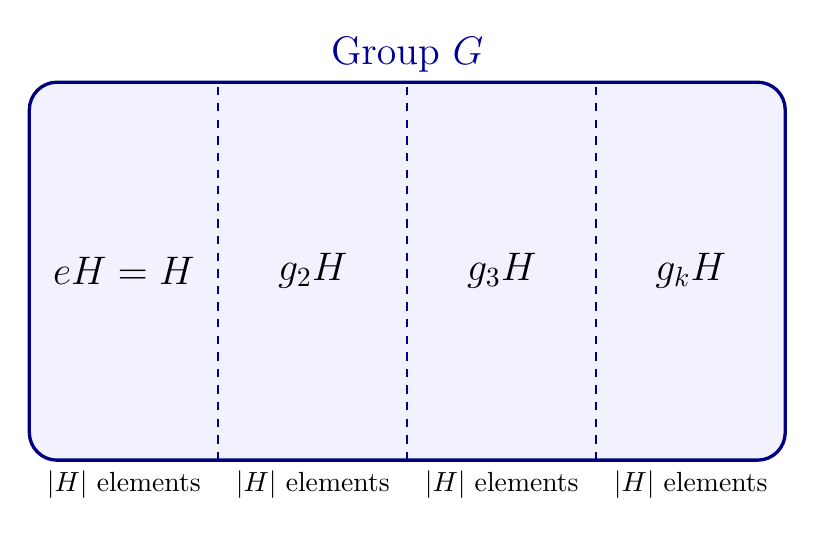
\begin{tikzpicture}[scale=1.2, thick]
        % 전체 군 G를 나타내는 큰 직사각형
        \draw[rounded corners=10pt, fill=blue!5, draw=blue!50!black, very thick] (0, 0) rectangle (8, 4);
        \node[above, font=\Large, text=blue!60!black] at (4, 4) {Group $G$};
        
        % 분할 선 긋기
        \draw[dashed, blue!50!black] (2, 0) -- (2, 4);
        \draw[dashed, blue!50!black] (4, 0) -- (4, 4);
        \draw[dashed, blue!50!black] (6, 0) -- (6, 4);
        
        % 각 코셋(Coset) 영역 라벨링
        \node[font=\Large] at (1, 2) {$eH = H$};
        \node[font=\Large] at (3, 2) {$g_2 H$};
        \node[font=\Large] at (5, 2) {$g_3 H$};
        \node[font=\Large] at (7, 2) {$g_k H$};
        
        % 각 코셋이 같은 크기(원소의 개수가 같음)임을 보여주는 설명
        \node[below] at (1, 0) {$|H|$ elements};
        \node[below] at (3, 0) {$|H|$ elements};
        \node[below] at (5, 0) {$|H|$ elements};
        \node[below] at (7, 0) {$|H|$ elements};
    \end{tikzpicture}
    \caption{A visual representation of Lagrange's Theorem foundation: The distinct left cosets perfectly partition the entire group $G$ into mutually disjoint subsets of identically equal size \cite{fraleigh}.}
    \label{fig:coset_partition}
\end{figure}



















% --- 부록 (Appendix) 시작 ---
\appendix
\section{The Division Algorithm}

The Division Algorithm is a fundamental theorem in number theory and abstract algebra. It serves as the logical mathematical foundation for understanding cyclic groups, greatest common divisors, and Euclidean domains \cite{dummit, gallian}. The rigorous proof of this theorem relies fundamentally on the Well-Ordering Principle of the integers.

\begin{theorem}[Well-Ordering Principle] \label{thm:wop}
Every non-empty subset of the non-negative integers contains a least element \cite{fraleigh}.
\end{theorem}

\begin{theorem}[The Division Algorithm] \label{thm:division}
Let $a$ and $b$ be integers with $b > 0$. Then there exist unique integers $q$ and $r$ such that 
\begin{equation}
    a = bq + r, \quad 0 \le r < b
\end{equation}
The integer $q$ is traditionally called the quotient, and $r$ is called the remainder \cite{fraleigh}.
\end{theorem}

\begin{proof}
\textbf{Existence:} \\
Consider the set $S$ defined by all non-negative remainders of the form $a - bk$ for any integer $k \in \mathbb{Z}$:
\begin{equation}
    S = \{ a - bk \mid k \in \mathbb{Z} \text{ and } a - bk \ge 0 \}
\end{equation}
First, we must formally show that $S$ is non-empty. 
If $a \ge 0$, choosing $k = 0$ yields $a - b(0) = a \ge 0$, which means $a \in S$. 
If $a < 0$, choosing $k = a$ yields $a - ba = a(1 - b)$. Since $b \ge 1$, we have $1 - b \le 0$. Multiplying two non-positive numbers gives $a(1 - b) \ge 0$, ensuring $a(1 - b) \in S$. 
Thus, $S$ is always a non-empty subset of the non-negative integers \cite{dummit}.

By the Well-Ordering Principle (Theorem \ref{thm:wop}), $S$ must contain a strictly least element. Let us denote this least element as $r$. Since $r \in S$, there exists some integer $q$ such that $r = a - bq$, which naturally rearranges to $a = bq + r$. Furthermore, by the very definition of $S$, $r \ge 0$ \cite{gallian}.

We must now prove that $r < b$. Suppose, for the sake of contradiction, that $r \ge b$. Then we can constructively define a new integer $r'$ such that:
\begin{equation}
    r' = r - b = (a - bq) - b = a - b(q + 1)
\end{equation}
Since $r \ge b$, it clearly follows that $r' \ge 0$. Furthermore, $r'$ is exactly of the form $a - bk$ (with $k = q + 1$), which dictates that $r' \in S$. However, $r' = r - b < r$ because $b > 0$. This directly contradicts our foundational assumption that $r$ is the least element of $S$ \cite{fraleigh}. Therefore, our assumption $r \ge b$ must be strictly false, conclusively proving that $0 \le r < b$.

\vspace{0.3cm}
\textbf{Uniqueness:} \\
To prove that $q$ and $r$ are algebraically unique, suppose there exist another pair of integers $q'$ and $r'$ satisfying the theorem:
\begin{equation}
    a = bq + r = bq' + r', \quad 0 \le r, r' < b
\end{equation}
Without loss of generality, we may assume $r \ge r'$. Subtracting the two algebraic equations yields:
\begin{equation}
    b(q - q') = r' - r \implies b \mid (r' - r)
\end{equation}
Since $0 \le r < b$ and $0 \le r' < b$, the difference $r' - r$ is strictly bounded by the inequality $-b < r' - r \le 0$. The only integer multiple of $b$ that strictly falls within this narrow range is $0$ \cite{dummit}. 

Therefore, $r' - r = 0$, which dictates $r = r'$. Substituting this result back into the prior equation gives $b(q - q') = 0$. Since $b > 0$, we are mathematically forced to conclude that $q = q'$. This completely proves that the quotient and the remainder are uniquely determined \cite{gallian}.
\end{proof}








\bibliographystyle{plain}
\bibliography{bibliography}

\end{document}